\section{บทที่ 6 การแปลงลาปลาซ}

\textbf{ชื่อบทภาษาอังกฤษ:} Laplace Transform\\
\textbf{รายวิชา:} คณิตศาสตร์วิศวกรรมไฟฟ้า (Electrical Engineering Mathematics)\\
\textbf{รหัสวิชา:} 5571102


\begin{quote}
\textbf{ขอบเขตของบท:} บทนี้ปูพื้นฐานการแปลงลาปลาซตั้งแต่นิยาม ตารางคู่การแปลง สมบัติ การแปลงผกผัน เศษส่วนย่อย ฟังก์ชันขั้นบันไดหนึ่งหน่วย ฟังก์ชันอิมพัลส์ การแก้สมการเชิงอนุพันธ์ และความสัมพันธ์กับระบบเชิงเส้น เพื่อเตรียมเข้าสู่บทที่ 7 ซึ่งจะประยุกต์ใช้กับวงจร RC, RL, RLC และฟังก์ชันถ่ายโอนอย่างเป็นระบบ
\end{quote}



\subsection{1. แนวคิดสำคัญของบท}

การแปลงลาปลาซ (Laplace Transform) เป็นเครื่องมือทางคณิตศาสตร์ที่เปลี่ยนปัญหาใน \textbf{โดเมนเวลา (time domain)} ซึ่งอาจอยู่ในรูปสมการเชิงอนุพันธ์ ให้กลายเป็นปัญหาเชิงพีชคณิตใน \textbf{โดเมนลาปลาซหรือโดเมน $s$ (Laplace domain / $s$-domain)} จากนั้นจึงแก้สมการในโดเมน $s$ และใช้การแปลงลาปลาซผกผันเพื่อกลับมาหาคำตอบในโดเมนเวลา

หัวใจสำคัญไม่ได้อยู่ที่การจำตารางเพียงอย่างเดียว แต่คือการมองเห็นว่า “การหาอนุพันธ์ในโดเมนเวลา” สามารถเปลี่ยนเป็น “การคูณด้วย $s$ พร้อมนำเงื่อนไขเริ่มต้นเข้ามารวมในสมการ” ได้ แนวคิดนี้มีคุณค่าอย่างมากในวิศวกรรมไฟฟ้า เพราะแรงดัน กระแส พลังงานสะสม และการตอบสนองของวงจรมักถูกอธิบายด้วยสมการเชิงอนุพันธ์

เมื่อพิจารณาระบบเชิงเส้นที่มีสัมประสิทธิ์คงที่ การแปลงลาปลาซช่วยให้ผู้เรียนสามารถ

\begin{itemize}
    \item รวมเงื่อนไขเริ่มต้นเข้ากับขั้นตอนการแก้สมการได้โดยตรง
    \item จัดการอินพุตที่เปลี่ยนค่าแบบทันทีด้วยฟังก์ชันขั้นบันไดหนึ่งหน่วย
    \item จัดการอินพุตแบบอิมพัลส์เชิงอุดมคติด้วยเดลตาของดิแรก
    \item ใช้เศษส่วนย่อยเพื่อเปลี่ยนฟังก์ชันตรรกยะในโดเมน $s$ กลับเป็นฟังก์ชันเวลา
    \item เชื่อมโยงสมการเชิงอนุพันธ์ การคอนโวลูชัน และแนวคิดระบบเชิงเส้นเข้าด้วยกัน
\end{itemize}

แหล่งอ้างอิงวิชาการที่ตรวจสอบบนเว็บ เช่น NIST Digital Library of Mathematical Functions และ MIT OpenCourseWare ให้รูปนิยาม สมบัติของอนุพันธ์ การคอนโวลูชัน และกระบวนการแก้สมการเชิงอนุพันธ์ด้วยลาปลาซในแนวทางเดียวกับที่ใช้ในบทนี้ ขณะที่ตำราวิศวกรรมคณิตศาสตร์มาตรฐานของ Kreyszig และตำราเฉพาะทางของ Fleisch ใช้การแปลงลาปลาซเป็นเครื่องมือพื้นฐานสำหรับฟิสิกส์และวิศวกรรม



\subsection{2. ความรู้พื้นฐานก่อนเรียน}

ก่อนเรียนบทนี้ นักศึกษาควรสามารถดำเนินการต่อไปนี้ได้ในระดับพื้นฐาน

\begin{enumerate}
    \item จัดรูปสมการพีชคณิตและแยกตัวประกอบพหุนามได้
    \item หารพหุนามและแยกเศษส่วนย่อยอย่างง่ายได้ หรือพร้อมทบทวนในบทนี้
    \item หาอนุพันธ์และปริพันธ์ของฟังก์ชันพื้นฐาน เช่น $e^{at}$, $\sin \omega t$, $\cos \omega t$ และ $t^n$
    \item แก้สมการเชิงอนุพันธ์อันดับหนึ่งและอันดับสองในกรณีพื้นฐาน หรืออย่างน้อยเข้าใจความหมายของอนุพันธ์และเงื่อนไขเริ่มต้น
    \item เข้าใจจำนวนเชิงซ้อนและรูป $s=\sigma+j\omega$ จากพื้นฐานจำนวนเชิงซ้อนในบทก่อนหน้า
    \item เข้าใจแนวคิดสัญญาณตามเวลา ฟังก์ชันเป็นคาบ และการแทนรูปคลื่นจากบทอนุกรมฟูเรียร์
\end{enumerate}

\begin{quote}
\textbf{ข้อเสนอแนะก่อนเริ่มสอน:} ใช้เวลา 10–15 นาทีทบทวนการแยกตัวประกอบพหุนามกำลังสองและการจัดรูปกำลังสองสมบูรณ์ เพราะเป็นทักษะที่มีผลโดยตรงต่อการหาลาปลาซผกผัน
\end{quote}



\subsection{3. คำสำคัญประจำบท}

\begin{table}[htbp]
    \centering
    \small
    \begin{tabularx}{\textwidth}{>{\raggedright\arraybackslash}p{0.26\textwidth} >{\raggedright\arraybackslash}p{0.25\textwidth} X}
        \hline
        \textbf{คำศัพท์ภาษาไทย} & \textbf{English} & \textbf{ความหมายโดยย่อ} \\
        \hline
        การแปลงลาปลาซ & Laplace Transform & การแปลงฟังก์ชันจากตัวแปรเวลา $t$ ไปเป็นฟังก์ชันของตัวแปรเชิงซ้อน $s$ \\
        โดเมนเวลา & Time Domain & การอธิบายสัญญาณหรือระบบในรูปฟังก์ชันของเวลา \\
        โดเมน $s$ & $s$-Domain & โดเมนหลังการแปลงลาปลาซ ใช้ตัวแปร $s=\sigma+j\omega$ \\
        การแปลงลาปลาซผกผัน & Inverse Laplace Transform & การเปลี่ยนจาก $F(s)$ กลับเป็น $f(t)$ \\
        บริเวณการลู่เข้า & Region of Convergence, ROC & ช่วงค่าของ $s$ ที่อินทิกรัลลาปลาซลู่เข้า \\
        สมบัติเชิงเส้น & Linearity & การแปลงผลบวกและค่าคงที่สามารถแยกทำทีละพจน์ได้ \\
        การเลื่อนในเวลา & Time Shifting & สมบัติที่เชื่อมการหน่วงเวลาเข้ากับตัวประกอบ $e^{-as}$ \\
        การเลื่อนในโดเมน $s$ & $s$-Shifting & สมบัติที่เชื่อมการคูณ $e^{at}$ ในเวลาเข้ากับการแทน $s-a$ \\
        เศษส่วนย่อย & Partial Fractions & วิธีแยกฟังก์ชันตรรกยะเป็นผลบวกของพจน์ที่หาลาปลาซผกผันได้ง่าย \\
        ฟังก์ชันขั้นบันไดหนึ่งหน่วย & Unit Step / Heaviside Function & ฟังก์ชันที่ใช้แทนการเปิดหรือเปลี่ยนอินพุต ณ เวลาที่กำหนด \\
        ฟังก์ชันอิมพัลส์ & Unit Impulse / Dirac Delta & แบบจำลองอุดมคติของอินพุตที่มีช่วงเวลาสั้นมากแต่พื้นที่รวมมีค่าจำกัด \\
        เงื่อนไขเริ่มต้น & Initial Conditions & ค่าของฟังก์ชันและอนุพันธ์ ณ จุดเริ่มต้นของการวิเคราะห์ \\
        ระบบเชิงเส้นไม่แปรตามเวลา & Linear Time-Invariant System, LTI & ระบบที่เป็นเชิงเส้นและสมบัติไม่เปลี่ยนตามการเลื่อนเวลา \\
        คอนโวลูชัน & Convolution & การรวมผลตอบสนองของระบบต่อองค์ประกอบย่อยของอินพุต \\
        \hline
    \end{tabularx}
\end{table}



\subsection{4. ผลลัพธ์การเรียนรู้ประจำบท}

เมื่อเรียนจบบทนี้ นักศึกษาสามารถ

\begin{enumerate}
    \item \textbf{อธิบาย} ความหมาย ความสำคัญ เงื่อนไขการลู่เข้า และบทบาทของการแปลงลาปลาซต่อการวิเคราะห์ปัญหาทางวิศวกรรมไฟฟ้าได้
    \item \textbf{คำนวณ} การแปลงลาปลาซของฟังก์ชันพื้นฐานโดยใช้นิยาม ตาราง และสมบัติที่เหมาะสมได้
    \item \textbf{หาการแปลงลาปลาซผกผัน} จากฟังก์ชันพื้นฐานและฟังก์ชันตรรกยะ โดยใช้การจัดรูปและวิธีเศษส่วนย่อยได้
    \item \textbf{แทนและวิเคราะห์} สัญญาณที่มีการเปิด-ปิดหรือเกิดแบบฉับพลันด้วยฟังก์ชันขั้นบันไดหนึ่งหน่วยและฟังก์ชันอิมพัลส์ได้
    \item \textbf{แก้สมการเชิงอนุพันธ์} ที่มีเงื่อนไขเริ่มต้นด้วยการแปลงลาปลาซ พร้อมตรวจสอบความสมเหตุสมผลของคำตอบได้
    \item \textbf{เชื่อมโยง} การแปลงลาปลาซกับระบบเชิงเส้น การคอนโวลูชัน และแนวคิดอินพุต–เอาต์พุตเพื่อเตรียมประยุกต์ใช้กับวงจรไฟฟ้าในบทถัดไปได้
\end{enumerate}

\subsubsection{4.1 ตารางเชื่อมโยง OBE: ผลลัพธ์–เนื้อหา–กิจกรรม–การประเมิน}

\begingroup
\hbadness=10000
\begin{table}[htbp]
    \centering
    \small
    \begin{tabularx}{\textwidth}{>{\raggedright\arraybackslash}p{0.18\textwidth} >{\raggedright\arraybackslash}p{0.15\textwidth} >{\raggedright\arraybackslash}p{0.23\textwidth} >{\raggedright\arraybackslash}p{0.17\textwidth} X}
        \hline
        \textbf{ผลลัพธ์การเรียนรู้ประจำบท} & \textbf{เนื้อหาที่เกี่ยวข้อง} & \textbf{กิจกรรมการเรียนรู้} & \textbf{วิธีประเมิน} & \textbf{หลักฐานการเรียนรู้} \\
        \hline
        CLO6.1 อธิบายความหมายและความสำคัญของลาปลาซ & 6.1–6.2, การลู่เข้า, โดเมน $s$ & วิเคราะห์แผนภาพ time domain $\to$ $s$-domain และอภิปรายความหมาย & คำถามปากเปล่า/แบบทดสอบสั้น & คำตอบอธิบายด้วยภาษาของตนเอง \\
        CLO6.2 คำนวณลาปลาซของฟังก์ชันพื้นฐาน & 6.2–6.4 & คำนวณจากนิยามและเปรียบเทียบกับตาราง & แบบฝึกหัดรายบุคคล & ขั้นตอนคำนวณและคำตอบ $F(s)$ \\
        CLO6.3 หาลาปลาซผกผันด้วยเศษส่วนย่อย & 6.5–6.6 & แยกกรณีรากต่างกัน รากซ้ำ และพจน์กำลังสอง & แบบฝึกหัดวิเคราะห์ & การจัดรูปและสัมประสิทธิ์เศษส่วนย่อยที่ถูกต้อง \\
        CLO6.4 วิเคราะห์ step/impulse & 6.7–6.8 & เขียนฟังก์ชันชิ้นส่วนให้อยู่ในรูป unit step และพิจารณา impulse & ใบงานสั้น & สมการสัญญาณและลาปลาซของสัญญาณ \\
        CLO6.5 แก้สมการเชิงอนุพันธ์ด้วยลาปลาซ & 6.9, 6.11 & แก้ IVP แบบเป็นขั้นตอนและตรวจค่าเริ่มต้น & แบบฝึกหัด/ข้อสอบอัตนัย & $Y(s)$, การแยกเศษส่วนย่อย, $y(t)$ และการตรวจสอบ \\
        CLO6.6 เชื่อมโยงกับระบบเชิงเส้น & 6.10 & วิเคราะห์ input–system–output และคอนโวลูชัน & คำถามเชิงวิเคราะห์/กรณีศึกษา & แผนภาพความสัมพันธ์และคำอธิบายเชิงระบบ \\
        \hline
    \end{tabularx}
\end{table}
\endgroup



\subsection{5. แผนผังเนื้อหาของบท}

\begin{center}
 ปัญหาในโดเมนเวลา\\
    v\\
นิยามการแปลงลาปลาซและเงื่อนไขการลู่เข้า\\
    v\\
ตารางคู่การแปลงพื้นฐาน\\
    v\\
สมบัติของการแปลงลาปลาซ\\
    v\\
การแปลงลาปลาซผกผัน\\
    v\\
การแยกเศษส่วนย่อย\\
    v\\
Unit Step และ Impulse\\
    v\\
แปลงสมการเชิงอนุพันธ์เป็นสมการพีชคณิตในโดเมน s\\
    v\\
แก้หา Y(s)\\
    v\\
Inverse Laplace -> y(t)\\
    v\\
เชื่อมโยงกับระบบเชิงเส้นและเตรียมเข้าสู่การวิเคราะห์วงจรในบทที่ 7\\
\end{center}

\subsection{6. บทนำ}

ในวิศวกรรมไฟฟ้า เรามักพบสมการที่มีอนุพันธ์ เช่น ความสัมพันธ์ของแรงดันตัวเก็บประจุ $i_C(t)=C\,dv_C(t)/dt$ หรือแรงดันตัวเหนี่ยวนำ $v_L(t)=L\,di_L(t)/dt$ เมื่อสร้างสมการวงจรจึงได้สมการเชิงอนุพันธ์ที่ต้องแก้พร้อมเงื่อนไขเริ่มต้น เช่น แรงดันเริ่มต้นของตัวเก็บประจุหรือกระแสเริ่มต้นของตัวเหนี่ยวนำ

ถ้าใช้วิธีในโดเมนเวลาโดยตรง ผู้เรียนต้องหาคำตอบทั่วไป แยกคำตอบธรรมชาติและคำตอบบังคับ แล้วคำนวณค่าคงที่จากเงื่อนไขเริ่มต้น วิธีนี้มีความสำคัญและควรเข้าใจ แต่เมื่ออินพุตเปลี่ยนแบบชิ้นส่วน มีการเปิดสวิตช์หลายครั้ง หรือมีอิมพัลส์ กระบวนการจะซับซ้อนขึ้นอย่างรวดเร็ว

การแปลงลาปลาซเสนออีกมุมมองหนึ่ง โดยแทนการดำเนินการ “หาอนุพันธ์” ด้วยการดำเนินการเชิงพีชคณิตในตัวแปร $s$ ทำให้สมการเชิงอนุพันธ์เชิงเส้นที่มีสัมประสิทธิ์คงที่สามารถเปลี่ยนเป็นสมการพหุนามหรือฟังก์ชันตรรกยะได้ MIT OpenCourseWare อธิบายแนวคิดนี้โดยตรงว่า Laplace transform เปลี่ยนสมการเชิงอนุพันธ์ของ $x(t)$ เป็นสมการพีชคณิตของ $X(s)$ แล้วจึงแปลงกลับเพื่อหาคำตอบในเวลา

สิ่งที่ผู้เรียนควรฝึกในบทนี้จึงมีสามระดับ

\begin{enumerate}
    \item \textbf{ระดับคู่การแปลง:} รู้ว่า $f(t)$ ใดสัมพันธ์กับ $F(s)$ ใด
    \item \textbf{ระดับสมบัติ:} ใช้ linearity, shifting, derivative rule และสมบัติอื่นเพื่อลดการคำนวณอินทิกรัลซ้ำ ๆ
    \item \textbf{ระดับการแก้ปัญหา:} เลือกวิธีจัดรูป $F(s)$ และใช้ inverse Laplace อย่างมีเหตุผล เพื่อกลับไปตีความในโดเมนเวลา
\end{enumerate}

\begin{quote}
\textbf{แนวคิดนำทาง:} การแปลงลาปลาซไม่ทำให้ฟิสิกส์ของระบบหายไป แต่เปลี่ยน “รูปภาษา” ที่ใช้เขียนปัญหา จากภาษาของอนุพันธ์ในเวลา ไปเป็นภาษาของพีชคณิตในตัวแปร $s$
\end{quote}



\section{7. เนื้อหาหลัก}

\subsection{7.1 ความหมายและความสำคัญของการแปลงลาปลาซ}

\subsubsection{\texorpdfstring{7.1.1 จากโดเมนเวลาไปสู่โดเมน $s$}{7.1.1 จากโดเมนเวลาไปสู่โดเมน s}}

ให้ $f(t)$ เป็นสัญญาณหรือฟังก์ชันในโดเมนเวลา การแปลงลาปลาซสร้างฟังก์ชันใหม่ $F(s)$ โดย $s$ เป็นจำนวนเชิงซ้อน

\[
s=\sigma+j\omega
\]

โดย

\begin{itemize}
    \item $\sigma$ คือส่วนจริงของ $s$ มีมิติเป็น $\mathrm{s}^{-1}$ เมื่อ $t$ วัดเป็นวินาที
    \item $\omega$ คือส่วนจินตภาพเชิงมุม มีมิติเป็น $\mathrm{rad/s}$ โดยเรเดียนถือเป็นมิติไร้หน่วยในเชิงมิติศาสตร์
    \item $j=\sqrt{-1}$
\end{itemize}

มองเชิงแนวคิด ปัจจัย $e^{-st}$ สามารถเขียนเป็น

\[
e^{-st}=e^{-\sigma t}e^{-j\omega t}
\]

ส่วน $e^{-\sigma t}$ ทำหน้าที่เป็นน้ำหนักเพิ่ม/ลดตามเวลา ส่วน $e^{-j\omega t}$ เชื่อมโยงกับพฤติกรรมเชิงสั่น ดังนั้น $F(s)$ จึงเก็บข้อมูลของ $f(t)$ ผ่านพารามิเตอร์เชิงซ้อน $s$

% [รูปที่ 1: แนวคิดการเปลี่ยนจากโดเมนเวลาไปสู่โดเมนลาปลาซ]
% ประเภทภาพ: Block Diagram / Technical Illustration
% ตำแหน่งที่แนะนำ: หลังหัวข้อ 7.1.1
% วัตถุประสงค์การเรียนรู้: ช่วยให้ผู้เรียนเห็นว่าการแปลงลาปลาซเปลี่ยนรูปการแทนปัญหา แต่ยังแทนระบบเดียวกัน
% คำอธิบายภาพ: ด้านซ้ายแสดงสัญญาณ $f(t)$ และสมการเชิงอนุพันธ์ในโดเมนเวลา ลูกศรผ่านบล็อก $\mathcal{L}\{\cdot\}$ ไปยังด้านขวาเป็น $F(s)$ และสมการพีชคณิต จากนั้นมีลูกศรย้อนกลับผ่าน $\mathcal{L}^{-1}\{\cdot\}$
% องค์ประกอบที่ต้องมี: time-domain waveform, differential equation, Laplace transform block, algebraic equation, inverse Laplace block, time-domain solution
% ข้อความหรือป้ายกำกับ: “โดเมนเวลา / Time Domain”, “การแปลงลาปลาซ / Laplace Transform”, “โดเมน s / s-Domain”, “การแปลงผกผัน / Inverse Laplace”
% ภาษาของป้ายกำกับ: ไทยและอังกฤษ
% สัดส่วนภาพ: 16:9
% Image Generation Prompt: Clean engineering mathematics textbook infographic showing a left-to-right transformation workflow. Left panel: a time-domain signal f(t) and a linear differential equation with derivatives. Center: a block labeled Laplace Transform L{·}. Right panel: F(s) and an algebraic equation in s. Add a reverse arrow through Inverse Laplace L^{-1}{·} back to the time-domain solution. White background, precise mathematical notation, bilingual Thai-English labels, clean vector style, 16:9.
% Alt Text: แผนภาพแสดงการแปลงปัญหาจากสมการเชิงอนุพันธ์ในโดเมนเวลาเป็นสมการพีชคณิตในโดเมน s และแปลงกลับเป็นคำตอบตามเวลา

\begin{figure}[htbp]
    \centering
    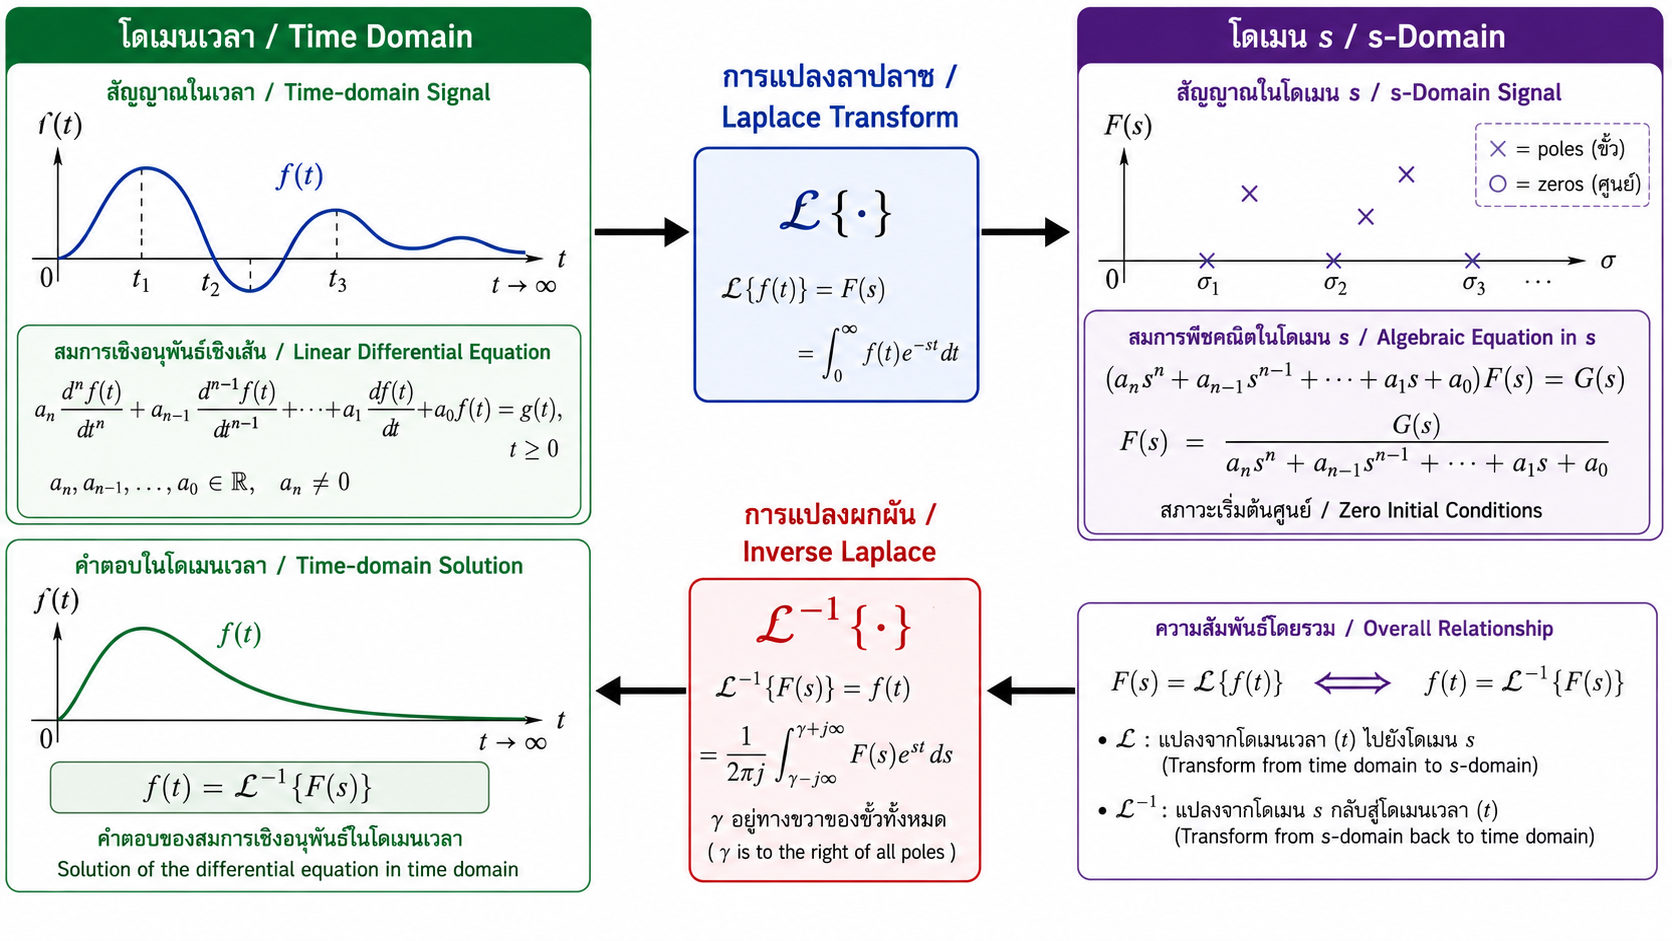
\includegraphics[width=0.8\textwidth]{images/chapter6/figure-01.png}
    \caption{แนวคิดการเปลี่ยนจากโดเมนเวลาไปสู่โดเมนลาปลาซ}
\end{figure}

\subsubsection{7.1.2 เหตุใดลาปลาซจึงเหมาะกับปัญหาวิศวกรรม}

การแปลงลาปลาซมีข้อเด่นเมื่อปัญหามีลักษณะต่อไปนี้

\begin{itemize}
    \item เป็นสมการเชิงอนุพันธ์เชิงเส้นที่มีสัมประสิทธิ์คงที่
    \item มีเงื่อนไขเริ่มต้นที่ต้องนำมาพิจารณา
    \item มีอินพุตแบบขั้นบันได พัลส์ หรืออิมพัลส์
    \item ต้องการมองความสัมพันธ์ระหว่างอินพุตและเอาต์พุตของระบบ
    \item ต้องการจัดการคอนโวลูชันให้กลายเป็นการคูณในโดเมน $s$
\end{itemize}

อย่างไรก็ตาม ลาปลาซไม่ใช่วิธีแทนทุกปัญหาโดยอัตโนมัติ หากระบบไม่เชิงเส้นอย่างรุนแรง สัมประสิทธิ์เปลี่ยนตามเวลา หรือฟังก์ชันไม่อยู่ในเงื่อนไขที่การแปลงลู่เข้า อาจต้องใช้วิธีอื่นร่วมด้วย

\subsubsection{\texorpdfstring{7.1.3 ข้อสังเกตเรื่องลาปลาซด้านเดียวและค่า ณ $t=0$}{7.1.3 ข้อสังเกตเรื่องลาปลาซด้านเดียวและค่า ณ t=0}}

ในงานวิศวกรรมมักใช้ \textbf{การแปลงลาปลาซด้านเดียว (unilateral Laplace transform)} เพื่อวิเคราะห์ระบบตั้งแต่เวลาเริ่มต้นและนำเงื่อนไขเริ่มต้นมารวมในสมการ ประเด็นที่ต้องระวังคือการตีความขอบล่างของอินทิกรัลและค่าที่ $t=0$ เมื่อมีความไม่ต่อเนื่องหรืออิมพัลส์ตรงจุดกำเนิด งานของ Lundberg, Miller และ Trumper ชี้ให้เห็นว่าการใช้สัญกรณ์ $0^-$ หรือ $0^+$ ต้องสอดคล้องกันเพื่อไม่ให้เกิดความขัดแย้งในการคำนวณอิมพัลส์และเงื่อนไขเริ่มต้น

\textbf{ข้อตกลงสำหรับบทนี้:}

\begin{itemize}
    \item สำหรับฟังก์ชันปกติที่ไม่มีอิมพัลส์ที่ $t=0$ ใช้นิยาม $\int_0^\infty f(t)e^{-st}dt$ ตามมาตรฐานทั่วไป
    \item เมื่อใช้สูตรอนุพันธ์ในโจทย์ค่าเริ่มต้น จะระบุค่าเริ่มต้นที่ใช้ให้ชัดเจน เช่น $f(0^-)$ สำหรับสถานะก่อนการสวิตช์ในบริบทวิศวกรรม หรือ $f(0^+)$ ตามนิยามทางคณิตศาสตร์ที่กำหนดไว้
    \item ไม่สลับอนุสัญญาระหว่างขั้นตอนของโจทย์เดียวกัน
\end{itemize}

ประเด็นนี้เป็น “วินัยด้านสัญกรณ์” ที่สำคัญกว่าการท่องจำสูตร



\subsection{7.2 นิยามของการแปลงลาปลาซ}

\subsubsection{7.2.1 นิยามพื้นฐาน}

สำหรับฟังก์ชัน $f(t)$ ที่นิยามเมื่อ $t\ge 0$ การแปลงลาปลาซเขียนได้เป็น

\[
\boxed{F(s)=\mathcal{L}\{f(t)\}=\int_{0}^{\infty} f(t)e^{-st}\,dt}
\]

\textbf{ที่มา:} นิยามนี้เป็นอินทิกรัลทรานส์ฟอร์มที่ใช้น้ำหนัก $e^{-st}$ รวมค่าของ $f(t)$ ตั้งแต่เวลาเริ่มต้นไปถึงอนันต์

\textbf{ความหมายของตัวแปร:}

\begin{itemize}
    \item $f(t)$ คือฟังก์ชันต้นฉบับในโดเมนเวลา
    \item $F(s)$ คือฟังก์ชันหลังการแปลงลาปลาซ
    \item $t$ คือเวลา โดยทั่วไปมีหน่วยวินาทีในงานไฟฟ้า
    \item $s$ คือความถี่เชิงซ้อน $s=\sigma+j\omega$ มีมิติ $\mathrm{s}^{-1}$
\end{itemize}

\textbf{หน่วย:} ถ้า $f(t)$ มีหน่วย $U$ และ $t$ มีหน่วยวินาที อินทิกรัลทำให้ $F(s)$ มีหน่วยโดยทั่วไปเป็น $U\cdot\mathrm{s}$ ทั้งนี้การตีความหน่วยต้องพิจารณาตามชนิดสัญญาณและนิยามระบบ

\textbf{สมมติฐานและเงื่อนไขการใช้:} ฟังก์ชันต้องทำให้อินทิกรัลลู่เข้าในช่วงค่าของ $s$ ที่สนใจ เงื่อนไขเพียงพอที่ใช้บ่อยคือฟังก์ชันเป็น piecewise continuous บนช่วงจำกัดและมีการเติบโตไม่เร็วกว่าฟังก์ชันเอกซ์โพเนนเชียลบางค่า

\subsubsection{7.2.2 เงื่อนไขการลู่เข้าและแนวคิด ROC}

ถ้ามีค่าคงที่ $M>0$ และ $\alpha$ ที่ทำให้

\[
|f(t)|\le Me^{\alpha t},\qquad t\ge 0
\]

แล้วการแปลงจะลู่เข้าสำหรับค่าของ $s$ ที่มีส่วนจริงมากพอ โดยทั่วไปในรูป

\[
\operatorname{Re}(s)>\alpha
\]

ช่วงค่าที่ลาปลาซลู่เข้าเรียกว่า \textbf{Region of Convergence (ROC)}

สำหรับบทนี้ ROC ใช้เพื่อสร้างความเข้าใจว่าฟังก์ชัน $F(s)$ ไม่ได้มีเพียงนิพจน์พีชคณิต แต่ยังมีเงื่อนไขของ $s$ ประกอบด้วย การวิเคราะห์ ROC เชิงลึกจะมีความสำคัญมากขึ้นในรายวิชาสัญญาณและระบบ

\subsubsection{\texorpdfstring{7.2.3 ตัวอย่างจากนิยาม: $f(t)=1$}{7.2.3 ตัวอย่างจากนิยาม: f(t)=1}}

\textbf{ตัวอย่างที่ 6.1 — ตัวอย่างพื้นฐาน}\\
จงหา $\mathcal{L}\{1\}$ จากนิยาม

\textbf{1) วิเคราะห์โจทย์} ต้องแทน $f(t)=1$ ลงในนิยามโดยตรง\\
\textbf{2) กำหนดตัวแปร} $t\ge 0$ และต้องเลือก $s$ ที่ทำให้อินทิกรัลลู่เข้า\\
\textbf{3) ใช้นิยาม}

\[
F(s)=\int_0^{\infty}e^{-st}\,dt
\]

\textbf{4) อินทิเกรต}

\[
F(s)=\left[-\frac{1}{s}e^{-st}\right]_0^{\infty}
\]

เมื่อ $\operatorname{Re}(s)>0$ จะมี $e^{-st}\to 0$ เมื่อ $t\to\infty$ ดังนั้น

\[
\boxed{\mathcal{L}\{1\}=\frac{1}{s}},\qquad \operatorname{Re}(s)>0
\]

\textbf{5) ตรวจสอบความสมเหตุสมผล} นิพจน์มีมิติของเวลา เพราะ $1/s$ มีหน่วยวินาทีเมื่อ $s$ มีหน่วย $\mathrm{s}^{-1}$\\
\textbf{6) แปลความหมาย} ฟังก์ชันคงที่ในเวลาเปลี่ยนเป็นฟังก์ชันที่แปรผกผันกับ $s$

\subsubsection{\texorpdfstring{7.2.4 ตัวอย่างจากนิยาม: $f(t)=e^{-3t}$}{7.2.4 ตัวอย่างจากนิยาม: f(t)=exp(-3t)}}

\textbf{ตัวอย่างที่ 6.2 — ตัวอย่างพื้นฐาน}\\
จงหา $\mathcal{L}\{e^{-3t}\}$

\[
\begin{aligned}
    F(s)&=\int_0^{\infty}e^{-3t}e^{-st}\,dt\\
    &=\int_0^{\infty}e^{-(s+3)t}\,dt
\end{aligned}
\]

อินทิกรัลลู่เข้าเมื่อ $\operatorname{Re}(s+3)>0$ หรือ $\operatorname{Re}(s)>-3$

\[
\begin{aligned}
    F(s)&=\left[-\frac{e^{-(s+3)t}}{s+3}\right]_0^{\infty}\\
    &=\frac{1}{s+3}
\end{aligned}
\]

จึงได้

\[
\boxed{\mathcal{L}\{e^{-3t}\}=\frac{1}{s+3}},\qquad \operatorname{Re}(s)>-3
\]

ตัวอย่างนี้แสดงให้เห็นว่าพจน์เอกซ์โพเนนเชียลในเวลาเกี่ยวข้องโดยตรงกับการเลื่อนตำแหน่งตัวประกอบเชิงเส้นในโดเมน $s$

% [รูปที่ 2: ผลของตัวประกอบน้ำหนัก $e^{-\sigma t}$ ต่อการลู่เข้าของอินทิกรัลลาปลาซ]
% ประเภทภาพ: Graph / Infographic
% ตำแหน่งที่แนะนำ: หลังหัวข้อ 7.2.4
% วัตถุประสงค์การเรียนรู้: ช่วยอธิบายว่าค่า $\sigma$ ที่มากขึ้นทำให้น้ำหนักลดลงเร็วขึ้นและเอื้อต่อการลู่เข้า
% คำอธิบายภาพ: กราฟเดียวแสดง $e^{-\sigma t}$ สำหรับ $\sigma=0.5,1,2$ บน $0\le t\le 6$ ทุกเส้นเริ่มที่ 1 และลดลงด้วยอัตราต่างกัน พร้อมลูกศร “larger $\sigma$ → faster decay”
% องค์ประกอบที่ต้องมี: แกน $t$ หน่วย s, แกน amplitude, legend ของ $\sigma$, จุดเริ่มต้นที่ 1
% ข้อความหรือป้ายกำกับ: “น้ำหนักเอกซ์โพเนนเชียล / Exponential Weighting”
% ภาษาของป้ายกำกับ: ไทยและอังกฤษ
% สัดส่วนภาพ: 16:9
% Image Generation Prompt: Engineering mathematics textbook graph showing exponential weighting functions exp(-sigma t) for sigma = 0.5, 1, and 2 over t from 0 to 6 seconds. All curves start at 1 and decay at different rates. Add a clear annotation that larger sigma gives faster decay and can improve convergence of the Laplace integral. White background, precise axes, bilingual Thai-English labels, clean vector style, 16:9.
% Graph Generation Prompt: Plot y=exp(-sigma*t) for sigma in {0.5,1,2}, t in [0,6] s. x-axis: time t (s). y-axis: weighting amplitude. Include legend and note “larger sigma → faster decay”.
% Alt Text: กราฟเปรียบเทียบฟังก์ชัน e ยกกำลังลบซิกมาตีสำหรับซิกมา 0.5, 1 และ 2 ซึ่งลดลงเร็วขึ้นเมื่อซิกมามากขึ้น

\begin{figure}[htbp]
    \centering
    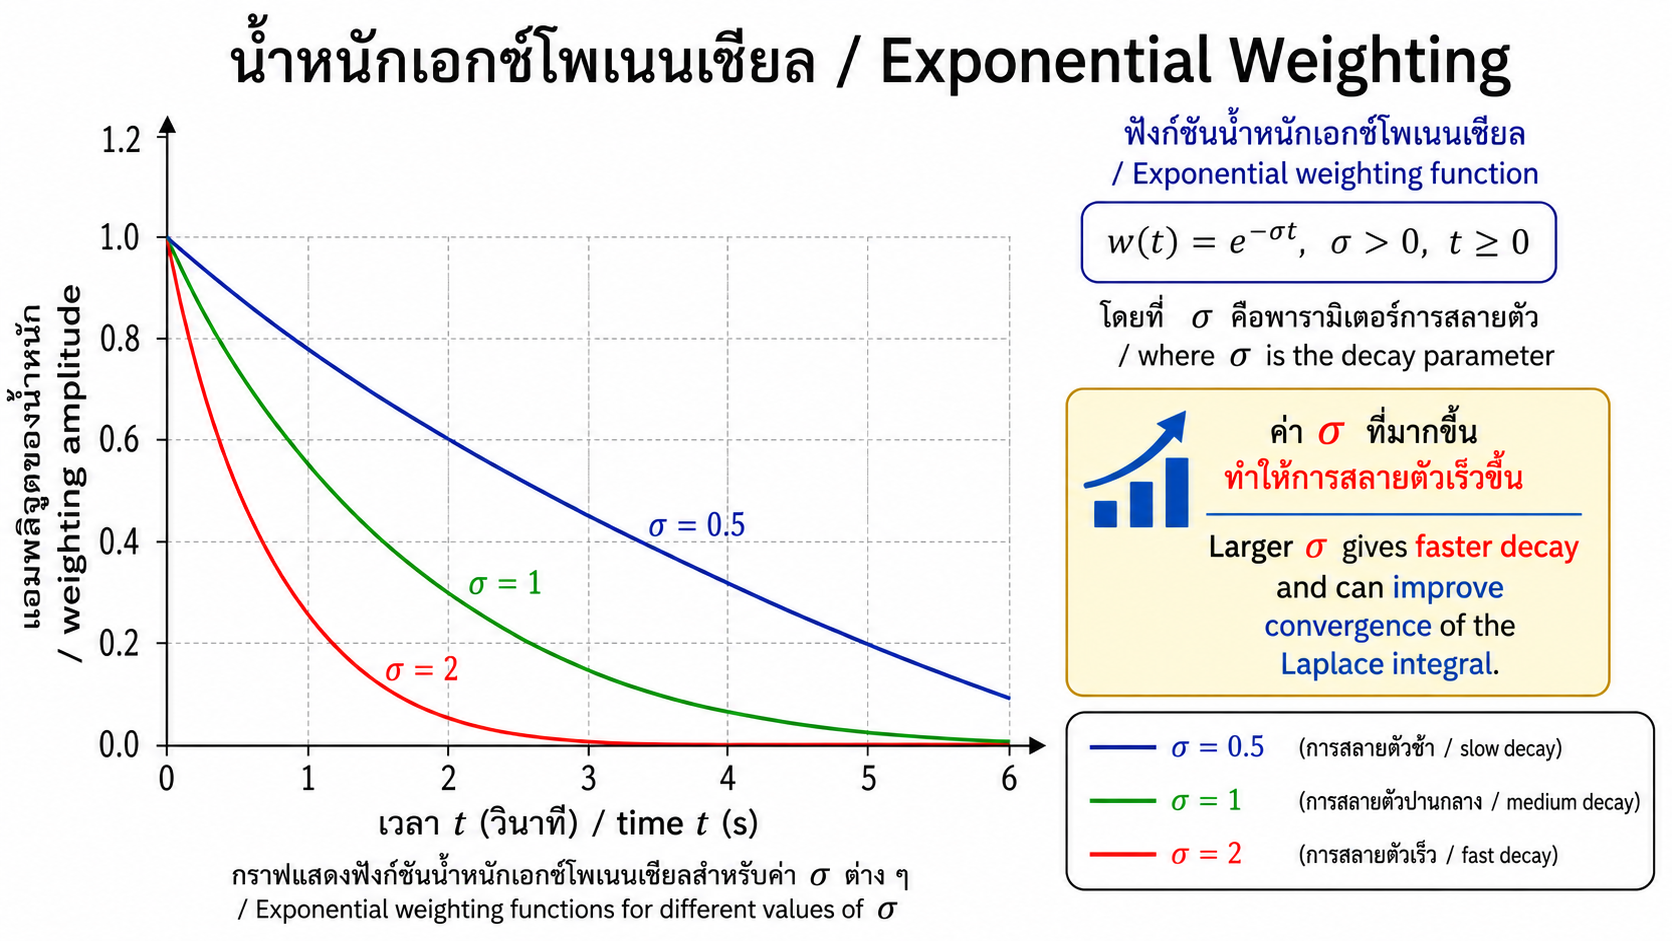
\includegraphics[width=0.8\textwidth]{images/chapter6/figure-02.png}
    \caption{ผลของตัวประกอบน้ำหนัก $e^{-\sigma t}$ ต่อการลู่เข้าของอินทิกรัลลาปลาซ}
\end{figure}



\subsection{7.3 ตารางการแปลงลาปลาซพื้นฐาน}

การใช้ตารางไม่ใช่การข้ามหลักการ แต่เป็นการนำคู่การแปลงที่พิสูจน์แล้วมาใช้ซ้ำอย่างมีประสิทธิภาพ ผู้เรียนควรจำ “รูปแบบสำคัญ” มากกว่าจำทุกบรรทัด และควรสามารถย้อนกลับไปพิสูจน์คู่พื้นฐานบางคู่จากนิยามได้

\subsubsection{ตารางที่ 6.1 คู่การแปลงลาปลาซที่ใช้บ่อย}

\begin{table}[htbp]
    \centering
    \begin{tabular}{r l l l}
        \hline
        \textbf{ลำดับ} & \textbf{$f(t)$} & \textbf{$F(s)=\mathcal{L}\{f(t)\}$} & \textbf{เงื่อนไข/ข้อสังเกต} \\
        \hline
        1 & $1$ & $\dfrac{1}{s}$ & $\operatorname{Re}(s)>0$ \\
        2 & $t$ & $\dfrac{1}{s^2}$ & $\operatorname{Re}(s)>0$ \\
        3 & $t^n$ & $\dfrac{n!}{s^{n+1}}$ & $n=0,1,2,\ldots$ \\
        4 & $e^{at}$ & $\dfrac{1}{s-a}$ & $\operatorname{Re}(s)>\operatorname{Re}(a)$ \\
        5 & $e^{-at}$ & $\dfrac{1}{s+a}$ & สำหรับ $a>0$ \\
        6 & $\sin \omega t$ & $\dfrac{\omega}{s^2+\omega^2}$ & $\omega$ มีหน่วย rad/s \\
        7 & $\cos \omega t$ & $\dfrac{s}{s^2+\omega^2}$ &  \\
        8 & $\sinh at$ & $\dfrac{a}{s^2-a^2}$ & ใช้เมื่ออยู่ในช่วงลู่เข้า \\
        9 & $\cosh at$ & $\dfrac{s}{s^2-a^2}$ &  \\
        10 & $u(t)$ & $\dfrac{1}{s}$ & สำหรับ unit step ที่เริ่มที่ศูนย์ \\
        11 & $u(t-a)$ & $\dfrac{e^{-as}}{s}$ & $a>0$ \\
        12 & $\delta(t)$ & $1$ & ภายใต้อนุสัญญาอิมพัลส์ที่จุดกำเนิดของการวิเคราะห์ \\
        13 & $\delta(t-a)$ & $e^{-as}$ & $a>0$ \\
        14 & $e^{-at}\sin \omega t$ & $\dfrac{\omega}{(s+a)^2+\omega^2}$ & จาก $s$-shifting \\
        15 & $e^{-at}\cos \omega t$ & $\dfrac{s+a}{(s+a)^2+\omega^2}$ & จาก $s$-shifting \\
        \hline
    \end{tabular}
\end{table}

\subsubsection{7.3.1 รูปแบบที่ควรจำเป็น “ครอบครัว”}

คู่การแปลงจำนวนมากสามารถจัดเป็นครอบครัวได้ เช่น

\begin{itemize}
    \item พหุนามเวลา $t^n$ $\leftrightarrow$ กำลังของ $1/s$
    \item เอกซ์โพเนนเชียล $e^{at}$ $\leftrightarrow$ ตัวประกอบ $1/(s-a)$
    \item ไซน์และโคไซน์ $\leftrightarrow$ พหุนามกำลังสอง $s^2+\omega^2$
    \item การหน่วงเวลา $\leftrightarrow$ ตัวคูณ $e^{-as}$
\end{itemize}

การจำแบบครอบครัวช่วยให้ผู้เรียนจัดรูป inverse Laplace ได้เร็วและลดความผิดพลาดจากการเทียบตารางแบบตรงตัว

\subsubsection{7.3.2 ตัวอย่างใช้ตารางแบบเชิงเส้น}

\textbf{ตัวอย่างที่ 6.3 — ตัวอย่างพื้นฐาน}\\
จงหา $\mathcal{L}\{2+3t-4e^{-2t}\}$

ใช้สมบัติเชิงเส้นและตาราง

\[
\begin{aligned}
    \mathcal{L}\{2+3t-4e^{-2t}\}&\\
    &=2\mathcal{L}\{1\}+3\mathcal{L}\{t\}-4\mathcal{L}\{e^{-2t}\}
\end{aligned}
\]

แทนค่าคู่การแปลง

\[
\boxed{F(s)=\frac{2}{s}+\frac{3}{s^2}-\frac{4}{s+2}}
\]

\textbf{ตรวจสอบ:} ทุกพจน์มีรูปที่สอดคล้องกับฟังก์ชันต้นฉบับ และไม่มีการรวมตัวส่วนโดยไม่จำเป็น เพราะรูปแยกพจน์เหมาะกับการอ่านความหมายและ inverse Laplace มากกว่า



\subsection{7.4 สมบัติของการแปลงลาปลาซ}

สมบัติทำหน้าที่เป็น “เครื่องมือแปลงรูป” ที่ช่วยหลีกเลี่ยงการอินทิเกรตจากนิยามทุกครั้ง

\subsubsection{7.4.1 สมบัติเชิงเส้น}

ถ้า

\[
\mathcal{L}\{f(t)\}=F(s),\qquad \mathcal{L}\{g(t)\}=G(s)
\]

แล้ว

\[
\boxed{\mathcal{L}\{af(t)+bg(t)\}=aF(s)+bG(s)}
\]

โดย $a,b$ เป็นค่าคงที่

\textbf{ที่มา:} เกิดจากสมบัติเชิงเส้นของอินทิกรัล\\
\textbf{เงื่อนไข:} $F(s)$ และ $G(s)$ ต้องลู่เข้าในบริเวณที่มีช่วงร่วมกัน\\
\textbf{ความหมายทางวิศวกรรม:} เป็นรากฐานของการใช้ superposition กับระบบเชิงเส้น

\subsubsection{\texorpdfstring{7.4.2 การเลื่อนในโดเมน $s$ (First Shifting Theorem)}{7.4.2 การเลื่อนในโดเมน s (First Shifting Theorem)}}

ถ้า $\mathcal{L}\{f(t)\}=F(s)$ แล้ว

\[
\boxed{\mathcal{L}\{e^{at}f(t)\}=F(s-a)}
\]

ตัวอย่างเช่น

\[
\begin{aligned}
    \mathcal{L}\{e^{-2t}\cos 3t\}&\\
    &=\frac{s+2}{(s+2)^2+9}
\end{aligned}
\]

\textbf{ความหมาย:} การคูณสัญญาณด้วยเอกซ์โพเนนเชียลในเวลาเลื่อนตัวแปรของฟังก์ชันลาปลาซ\\
\textbf{ข้อจำกัด:} ต้องปรับ ROC ให้สอดคล้องกับการเลื่อน

\subsubsection{7.4.3 การเลื่อนเวลา (Second Shifting Theorem)}

ถ้า $a>0$ และ $\mathcal{L}\{f(t)\}=F(s)$ แล้ว

\[
\boxed{\mathcal{L}\{u(t-a)f(t-a)\}=e^{-as}F(s)}
\]

สมบัตินี้สำคัญมากสำหรับอินพุตที่เริ่มทำงานภายหลัง เช่น เปิดแหล่งจ่ายเมื่อ $t=2\,\mathrm{s}$

\subsubsection{7.4.4 ลาปลาซของอนุพันธ์อันดับหนึ่ง}

สำหรับฟังก์ชันที่มีความต่อเนื่องเพียงพอ

\[
\boxed{\mathcal{L}\{f'(t)\}=sF(s)-f(0)}
\]

เมื่อใช้งานกับโจทย์สวิตชิง ต้องระบุว่า $f(0)$ หมายถึง $f(0^-)$ หรือ $f(0^+)$ ตามอนุสัญญาที่เลือก

\textbf{ที่มาโดยย่อ:} ใช้ integration by parts กับนิยามของลาปลาซ

ให้ $u=e^{-st}$ และ $dv=f'(t)dt$ จะได้

\[
\begin{aligned}
    \int_0^\infty e^{-st}f'(t)dt&\\
    &=\left[e^{-st}f(t)\right]_0^\infty+s\int_0^\infty e^{-st}f(t)dt
\end{aligned}
\]

ภายใต้เงื่อนไขที่พจน์ขอบเขตที่อนันต์เป็นศูนย์ จึงได้สูตรข้างต้น

\textbf{ความหมายทางวิศวกรรม:} เงื่อนไขเริ่มต้นปรากฏขึ้นในสมการหลังแปลงโดยอัตโนมัติ นี่คือเหตุผลสำคัญที่ลาปลาซเหมาะกับ initial-value problems

\subsubsection{\texorpdfstring{7.4.5 ลาปลาซของอนุพันธ์อันดับ $n$}{7.4.5 ลาปลาซของอนุพันธ์อันดับ n}}

\[
\boxed{\mathcal{L}\{f^{(n)}(t)\} =s^nF(s)-s^{n-1}f(0)-s^{n-2}f'(0)-\cdots-f^{(n-1)}(0)}
\]

สำหรับอันดับสอง

\[
\mathcal{L}\{f''(t)\}=s^2F(s)-sf(0)-f'(0)
\]

สูตรนี้จะถูกใช้ซ้ำในการแก้สมการเชิงอนุพันธ์อันดับสอง

\subsubsection{7.4.6 ลาปลาซของปริพันธ์ตามเวลา}

ถ้า

\[
g(t)=\int_0^t f(\tau)d\tau
\]

แล้ว

\[
\boxed{\mathcal{L}\{g(t)\}=\frac{F(s)}{s}}
\]

การอินทิเกรตในโดเมนเวลาเทียบได้กับการหารด้วย $s$ ในโดเมนลาปลาซภายใต้เงื่อนไขที่เหมาะสม

\subsubsection{\texorpdfstring{7.4.7 การคูณด้วย $t$}{7.4.7 การคูณด้วย t}}

\[
\boxed{\mathcal{L}\{t f(t)\}=-\frac{dF(s)}{ds}}
\]

ทั่วไป

\[
\boxed{\mathcal{L}\{t^n f(t)\}=(-1)^n\frac{d^nF(s)}{ds^n}}
\]

สมบัตินี้ช่วยสร้างคู่การแปลงใหม่โดยไม่ต้องอินทิเกรตจากนิยาม

\subsubsection{7.4.8 ฟังก์ชันเป็นคาบ}

ถ้า $f(t+T)=f(t)$ สำหรับ $T>0$ แล้ว

\[
\boxed{\mathcal{L}\{f(t)\} =\frac{\displaystyle\int_0^T e^{-st}f(t)dt}{1-e^{-sT}}}
\]

สมบัตินี้เชื่อมโยงบทลาปลาซกับพื้นฐานฟังก์ชันเป็นคาบจากบทฟูเรียร์ แต่เป้าหมายต่างกัน: อนุกรมฟูเรียร์มุ่งแยกองค์ประกอบความถี่ของสัญญาณเป็นคาบ ขณะที่ลาปลาซมุ่งสร้างตัวแทนในโดเมนเชิงซ้อนเพื่อวิเคราะห์สมการและระบบ

\subsubsection{7.4.9 ทฤษฎีค่าเริ่มต้นและค่าสุดท้าย}

ภายใต้เงื่อนไขที่เหมาะสม

\[
\boxed{f(0^+)=\lim_{s\to\infty}sF(s)}
\]

และสำหรับกรณีที่ลิมิตค่าสุดท้ายมีอยู่และระบบไม่มีพฤติกรรมที่ทำให้คำตอบไม่ลู่เข้าสู่ค่าคงที่

\[
\boxed{\lim_{t\to\infty}f(t)=\lim_{s\to 0}sF(s)}
\]

\begin{quote}
\textbf{ข้อควรระวัง:} Final Value Theorem ไม่ควรใช้แบบกลไกกับสัญญาณที่ไม่ลู่เข้าสู่ค่าคงที่ เช่น การสั่นคงอยู่หรือระบบที่มีพฤติกรรมไม่เสถียร การตรวจเงื่อนไขของโพลอย่างละเอียดจะเชื่อมโยงกับบทถัดไป
\end{quote}

\subsubsection{ตารางที่ 6.2 สรุปสมบัติสำคัญ}

\begin{table}[htbp]
    \centering
    \begin{tabular}{l l l l}
        \hline
        \textbf{สมบัติ} & \textbf{เวลา} & \textbf{โดเมน $s$} & \textbf{ใช้เมื่อ} \\
        \hline
        Linearity & $af+bg$ & $aF+bG$ & แยกหลายพจน์ \\
        $s$-shift & $e^{at}f(t)$ & $F(s-a)$ & มีเอกซ์โพเนนเชียลคูณ \\
        time shift & $u(t-a)f(t-a)$ & $e^{-as}F(s)$ & อินพุตเริ่มช้า \\
        derivative & $f'(t)$ & $sF-f(0)$ & ODE อันดับหนึ่ง \\
        second derivative & $f''(t)$ & $s^2F-sf(0)-f'(0)$ & ODE อันดับสอง \\
        integration & $\int_0^t f(\tau)d\tau$ & $F(s)/s$ & ระบบสะสม \\
        multiply by $t$ & $tf(t)$ & $-F'(s)$ & สร้างคู่การแปลงใหม่ \\
        convolution & $(f*g)(t)$ & $F(s)G(s)$ & ระบบ LTI / impulse response \\
        \hline
    \end{tabular}
\end{table}



\subsection{7.5 การแปลงลาปลาซผกผัน}

การแปลงลาปลาซผกผันเขียนเป็น

\[
\boxed{f(t)=\mathcal{L}^{-1}\{F(s)\}}
\]

ในทางทฤษฎีมีสูตรอินทิกรัลผกผันเชิงซ้อน แต่สำหรับงานวิศวกรรมระดับต้น การหาลาปลาซผกผันส่วนใหญ่ทำโดย

\begin{enumerate}
    \item เทียบตารางโดยตรง
    \item จัดรูปกำลังสองสมบูรณ์
    \item ใช้ shifting theorem
    \item แยกเศษส่วนย่อย
\end{enumerate}

MIT OpenCourseWare ระบุอย่างชัดเจนว่ากลวิธีหลักสำหรับ inverse Laplace ในระดับนี้คือ table lookup และ partial fractions

\subsubsection{7.5.1 ตัวอย่างการจัดรูปกำลังสองสมบูรณ์}

\textbf{ตัวอย่างที่ 6.4 — ตัวอย่างเชิงวิเคราะห์}\\
จงหา

\[
\mathcal{L}^{-1}\left\{\frac{2s+5}{s^2+4s+13}\right\}
\]

\textbf{1) วิเคราะห์ตัวส่วน}

\[
s^2+4s+13=(s+2)^2+9
\]

\textbf{2) จัดตัวเศษให้สัมพันธ์กับ $s+2$}

\[
2s+5=2(s+2)+1
\]

ดังนั้น

\[
\begin{aligned}
    F(s)&=\frac{2(s+2)}{(s+2)^2+3^2}\\
    &\quad +\frac{1}{(s+2)^2+3^2}
\end{aligned}
\]

\textbf{3) เทียบตาราง}

\[
\begin{aligned}
    \mathcal{L}^{-1}\left\{\frac{s+a}{(s+a)^2+\omega^2}\right\}&\\
    &=e^{-at}\cos\omega t
\end{aligned}
\]

และ

\[
\begin{aligned}
    \mathcal{L}^{-1}\left\{\frac{\omega}{(s+a)^2+\omega^2}\right\}&\\
    &=e^{-at}\sin\omega t
\end{aligned}
\]

พจน์ที่สองต้องทำให้มี $3$ ที่ตัวเศษ

\[
\begin{aligned}
    \frac{1}{(s+2)^2+9}&\\
    &=\frac{1}{3}\frac{3}{(s+2)^2+9}
\end{aligned}
\]

จึงได้

\[
\boxed{f(t)=2e^{-2t}\cos 3t+\frac{1}{3}e^{-2t}\sin 3t}
\]

\textbf{ตรวจสอบ:} รูปคำตอบเป็นไซน์และโคไซน์ที่ถูกคูณด้วยเอกซ์โพเนนเชียลลดลง ซึ่งสอดคล้องกับตัวส่วนที่เป็นกำลังสองสมบูรณ์เลื่อนด้วย $s+2$



\subsection{7.6 การใช้เศษส่วนย่อยในการหาลาปลาซผกผัน}

ถ้า $F(s)$ เป็นฟังก์ชันตรรกยะ

\[
F(s)=\frac{N(s)}{D(s)}
\]

และดีกรีของ $N(s)$ น้อยกว่าดีกรีของ $D(s)$ สามารถแยก $F(s)$ เป็นผลบวกของพจน์ที่เทียบตารางได้ง่าย

ถ้าดีกรีตัวเศษมากกว่าหรือเท่ากับตัวส่วน ต้อง \textbf{หารพหุนามก่อน}

\subsubsection{7.6.1 กรณีตัวประกอบเชิงเส้นไม่ซ้ำ}

ถ้า

\[
D(s)=(s-a)(s-b)
\]

เขียน

\[
F(s)=\frac{A}{s-a}+\frac{B}{s-b}
\]

\subsubsection{7.6.2 กรณีตัวประกอบเชิงเส้นซ้ำ}

ถ้า

\[
D(s)=(s-a)^m
\]

ต้องเขียนทุกกำลัง

\[
\frac{A_1}{s-a}+\frac{A_2}{(s-a)^2}+\cdots+\frac{A_m}{(s-a)^m}
\]

\subsubsection{7.6.3 กรณีตัวประกอบกำลังสองที่แยกตัวประกอบจริงไม่ได้}

ถ้า

\[
D(s)=s^2+bs+c
\]

และไม่แยกเป็นรากจริง ควรจัดเป็นกำลังสองสมบูรณ์และใช้ตัวเศษเชิงเส้น

\[
\frac{As+B}{s^2+bs+c}
\]

จากนั้นจัดให้เทียบกับรูปไซน์/โคไซน์

\subsubsection{ตารางที่ 6.3 รูปแบบเศษส่วนย่อยที่พบบ่อย}

\begin{table}[htbp]
    \centering
    \begin{tabular}{l l}
        \hline
        \textbf{ลักษณะตัวส่วน} & \textbf{รูปที่ต้องตั้ง} \\
        \hline
        $(s+a)(s+b)$ & $\dfrac{A}{s+a}+\dfrac{B}{s+b}$ \\
        $(s+a)^2$ & $\dfrac{A}{s+a}+\dfrac{B}{(s+a)^2}$ \\
        $(s+a)^3$ & $\dfrac{A}{s+a}+\dfrac{B}{(s+a)^2}+\dfrac{C}{(s+a)^3}$ \\
        $(s+a)(s^2+bs+c)$ & $\dfrac{A}{s+a}+\dfrac{Bs+C}{s^2+bs+c}$ \\
        \hline
    \end{tabular}
\end{table}

\subsubsection{7.6.4 ตัวอย่างรากเชิงเส้นไม่ซ้ำ}

\textbf{ตัวอย่างที่ 6.5 — ตัวอย่างเชิงวิเคราะห์}\\
จงหา

\[
\mathcal{L}^{-1}\left\{\frac{3s+7}{s(s+1)(s+2)}\right\}
\]

\textbf{1) ตั้งเศษส่วนย่อย}

\[
\begin{aligned}
    \frac{3s+7}{s(s+1)(s+2)}&\\
    &=\frac{A}{s}+\frac{B}{s+1}+\frac{C}{s+2}
\end{aligned}
\]

\textbf{2) หา $A$ โดยแทน $s=0$}

\[
A=\frac{7}{(1)(2)}=\frac{7}{2}
\]

\textbf{3) หา $B$ โดยแทน $s=-1$}

\[
B=\frac{3(-1)+7}{(-1)(1)}=-4
\]

\textbf{4) หา $C$ โดยแทน $s=-2$}

\[
C=\frac{3(-2)+7}{(-2)(-1)}=\frac{1}{2}
\]

ดังนั้น

\[
F(s)=\frac{7/2}{s}-\frac{4}{s+1}+\frac{1/2}{s+2}
\]

ใช้ inverse Laplace ทีละพจน์

\[
\boxed{f(t)=\frac{7}{2}-4e^{-t}+\frac{1}{2}e^{-2t}}
\]

\textbf{ตรวจสอบค่าเริ่มต้น:} $f(0^+)=3.5-4+0.5=0$ ซึ่งสอดคล้องกับพฤติกรรมที่ได้จาก $\lim_{s\to\infty}sF(s)=0$

\subsubsection{7.6.5 ตัวอย่างรากซ้ำ}

\textbf{ตัวอย่างที่ 6.6 — ตัวอย่างเชิงวิเคราะห์}\\
จงหา

\[
\mathcal{L}^{-1}\left\{\frac{s+3}{s(s+1)^2}\right\}
\]

ตั้ง

\[
\begin{aligned}
    \frac{s+3}{s(s+1)^2}&\\
    &=\frac{A}{s}+\frac{B}{s+1}+\frac{C}{(s+1)^2}
\end{aligned}
\]

คูณด้วย $s(s+1)^2$

\[
s+3=A(s+1)^2+Bs(s+1)+Cs
\]

แทน $s=0$ ได้ $A=3$

เทียบสัมประสิทธิ์หรือจัดรูป จะได้

\[
B=-3,\qquad C=-2
\]

ดังนั้น

\[
F(s)=\frac{3}{s}-\frac{3}{s+1}-\frac{2}{(s+1)^2}
\]

โดย

\[
\mathcal{L}^{-1}\left\{\frac{1}{(s+1)^2}\right\}=te^{-t}
\]

จึงได้

\[
\boxed{f(t)=3-3e^{-t}-2te^{-t}}
\]

% [รูปที่ 3: ขั้นตอนเลือกวิธีหาลาปลาซผกผันและเศษส่วนย่อย]
% ประเภทภาพ: Flowchart
% ตำแหน่งที่แนะนำ: หลังตัวอย่าง 6.6
% วัตถุประสงค์การเรียนรู้: ให้ผู้เรียนเลือกวิธีได้อย่างเป็นระบบแทนการลองผิดลองถูก
% คำอธิบายภาพ: เริ่มจาก F(s) → เทียบตารางได้หรือไม่ → ถ้าไม่ได้ตรวจว่าเป็น rational function หรือไม่ → ดีกรีเศษ < ส่วนหรือไม่ → หารพหุนามถ้าจำเป็น → factor denominator → เลือกรูป distinct/repeated/quadratic → solve coefficients → inverse by table
% องค์ประกอบที่ต้องมี: decision diamonds, partial fraction branches, final verification
% ข้อความหรือป้ายกำกับ: “Table lookup”, “Polynomial division”, “Distinct roots”, “Repeated roots”, “Quadratic factor”, “Verify” พร้อมภาษาไทย
% ภาษาของป้ายกำกับ: ไทยและอังกฤษ
% สัดส่วนภาพ: 16:9
% Image Generation Prompt: Clean engineering mathematics decision flowchart for inverse Laplace transforms. Start with F(s), ask whether direct table lookup is possible. If not, determine whether it is a rational function, whether polynomial division is required, factor the denominator, branch to distinct linear factors, repeated linear factors, or irreducible quadratic factors, solve coefficients, apply inverse Laplace table, then verify. Bilingual Thai-English labels, white background, precise vector textbook style, 16:9.
% Alt Text: ผังงานแสดงขั้นตอนเลือกวิธีหาลาปลาซผกผัน ตั้งแต่เทียบตาราง การหารพหุนาม การแยกตัวประกอบ การทำเศษส่วนย่อย จนถึงการตรวจสอบคำตอบ

\begin{figure}[htbp]
    \centering
    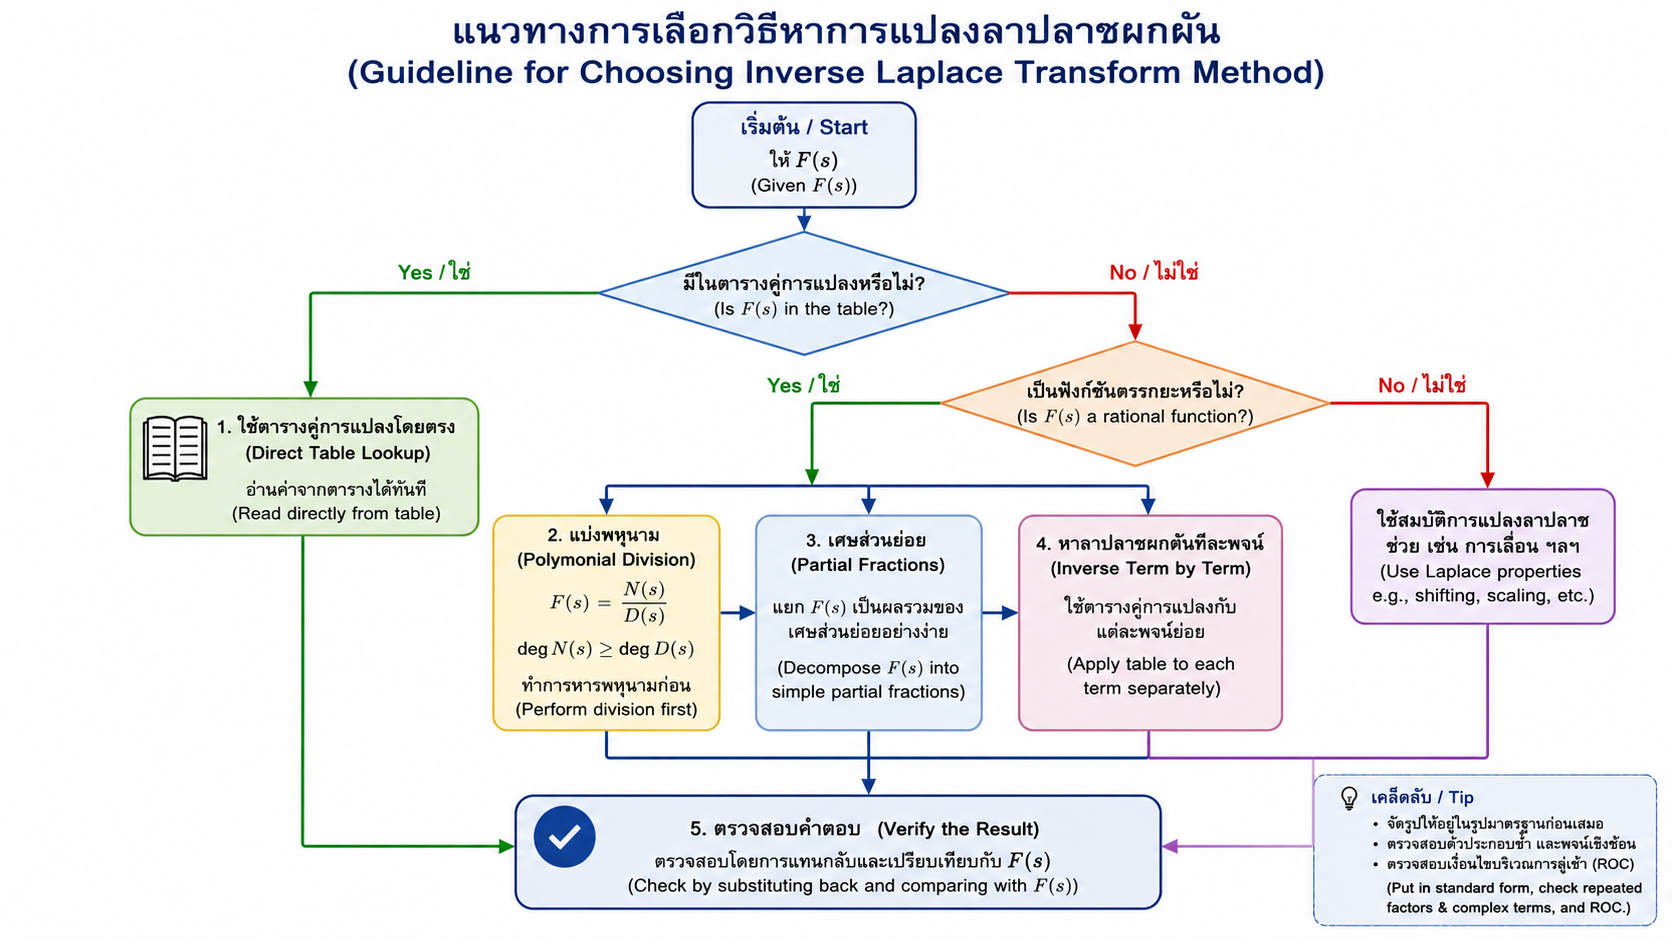
\includegraphics[width=0.8\textwidth]{images/chapter6/figure-03.png}
    \caption{ขั้นตอนเลือกวิธีหาลาปลาซผกผันและเศษส่วนย่อย}
\end{figure}



\subsection{7.7 ฟังก์ชันขั้นบันไดหนึ่งหน่วย}

\subsubsection{7.7.1 นิยาม Unit Step}

ฟังก์ชันขั้นบันไดหนึ่งหน่วยหรือ Heaviside function ใช้แทนเหตุการณ์ที่ “เปิด” ณ เวลาหนึ่ง เขียนได้ว่า

\[
u(t-a)=
\begin{cases}
0, & t<a\\
1, & t>a
\end{cases}
\]

ค่าที่จุด $t=a$ เพียงจุดเดียวมักไม่กระทบต่ออินทิกรัลธรรมดา แต่เมื่อเชื่อมโยงกับ generalized functions ต้องรักษาอนุสัญญาให้สอดคล้องกัน

สำหรับ $a=0$

\[
\mathcal{L}\{u(t)\}=\frac{1}{s}
\]

และสำหรับ unit step ที่หน่วงเวลา

\[
\boxed{\mathcal{L}\{u(t-a)\}=\frac{e^{-as}}{s}}
\]

\textbf{ความหมายของตัวแปร:} $a$ คือเวลาที่สัญญาณเริ่มทำงาน มีหน่วยเดียวกับ $t$\\
\textbf{ความหมายทางกายภาพ:} ในวงจรไฟฟ้า $u(t-a)$ สามารถใช้แทนการปิดสวิตช์หรือจ่ายแรงดันเมื่อถึงเวลา $a$

\subsubsection{7.7.2 การเขียนฟังก์ชันแบบชิ้นส่วนด้วย Unit Step}

สมมติสัญญาณ

\[
f(t)=
\begin{cases}
0, & 0\le t<2\\
t-2, & t\ge 2
\end{cases}
\]

เขียนได้เป็น

\[
f(t)=(t-2)u(t-2)
\]

ใช้ time-shifting theorem โดยให้ $g(t)=t$ และ $G(s)=1/s^2$

\[
\boxed{F(s)=e^{-2s}\frac{1}{s^2}}
\]

การเขียนในรูป $u(t-a)f(t-a)$ มีความสำคัญ เพราะสูตรเลื่อนเวลาต้องการฟังก์ชันภายในที่เขียนด้วยตัวแปร “นับจากจุดที่เริ่ม” เช่น $t-a$

\subsubsection{7.7.3 พัลส์สี่เหลี่ยมด้วยผลต่างของ Unit Step}

สัญญาณที่มีค่า 5 ตั้งแต่ $t=1$ ถึง $t=3$ และเป็นศูนย์ช่วงอื่น เขียนได้เป็น

\[
f(t)=5[u(t-1)-u(t-3)]
\]

ดังนั้น

\[
\boxed{F(s)=\frac{5}{s}\left(e^{-s}-e^{-3s}\right)}
\]

\textbf{การแปลความหมาย:} ตัวคูณ $e^{-s}$ และ $e^{-3s}$ แสดงเวลาเริ่มและเวลาสิ้นสุดของพัลส์โดยตรงในโดเมน $s$

% [รูปที่ 4: Unit Step และพัลส์สี่เหลี่ยมจากผลต่างของ Unit Step]
% ประเภทภาพ: Graph / Technical Illustration
% ตำแหน่งที่แนะนำ: หลังหัวข้อ 7.7.3
% วัตถุประสงค์การเรียนรู้: ให้ผู้เรียนเชื่อมกราฟสัญญาณแบบชิ้นส่วนกับสมการ unit step
% คำอธิบายภาพ: แบ่งเป็นสองแผง แผงบนแสดง $u(t-a)$ ที่กระโดดจาก 0 เป็น 1 ที่ $t=a$ แผงล่างแสดงพัลส์ $5[u(t-1)-u(t-3)]$ มีระดับ 5 ระหว่าง 1 ถึง 3 วินาที
% องค์ประกอบที่ต้องมี: แกนเวลา, ระดับแอมพลิจูด, เส้นประที่ $t=a$, $t=1$, $t=3$, สมการกำกับ
% ข้อความหรือป้ายกำกับ: “เปิด / Turn-on”, “ปิด / Turn-off”, “Unit Step”, “Rectangular Pulse”
% ภาษาของป้ายกำกับ: ไทยและอังกฤษ
% สัดส่วนภาพ: 16:9
% Image Generation Prompt: Two-panel engineering mathematics graph on a white background. Top panel: delayed unit step u(t-a), zero before t=a and one after t=a, with a vertical dashed line at t=a. Bottom panel: rectangular pulse 5[u(t-1)-u(t-3)], amplitude 5 between 1 and 3 seconds and zero elsewhere. Include precise axes, equations, bilingual Thai-English labels, clean vector textbook style, 16:9.
% Graph Generation Prompt: Top: y=0 for t<a and y=1 for t>a. Bottom: y=5 for 1<=t<3 and 0 otherwise. x-axis time t (s), y-axis amplitude. Mark t=a, 1 s, and 3 s.
% Alt Text: กราฟด้านบนแสดงขั้นบันไดหนึ่งหน่วยที่เริ่มที่เวลา a และกราฟด้านล่างแสดงพัลส์ระดับ 5 จากเวลา 1 ถึง 3 วินาทีซึ่งสร้างจากผลต่างของ unit step

\begin{figure}[htbp]
    \centering
    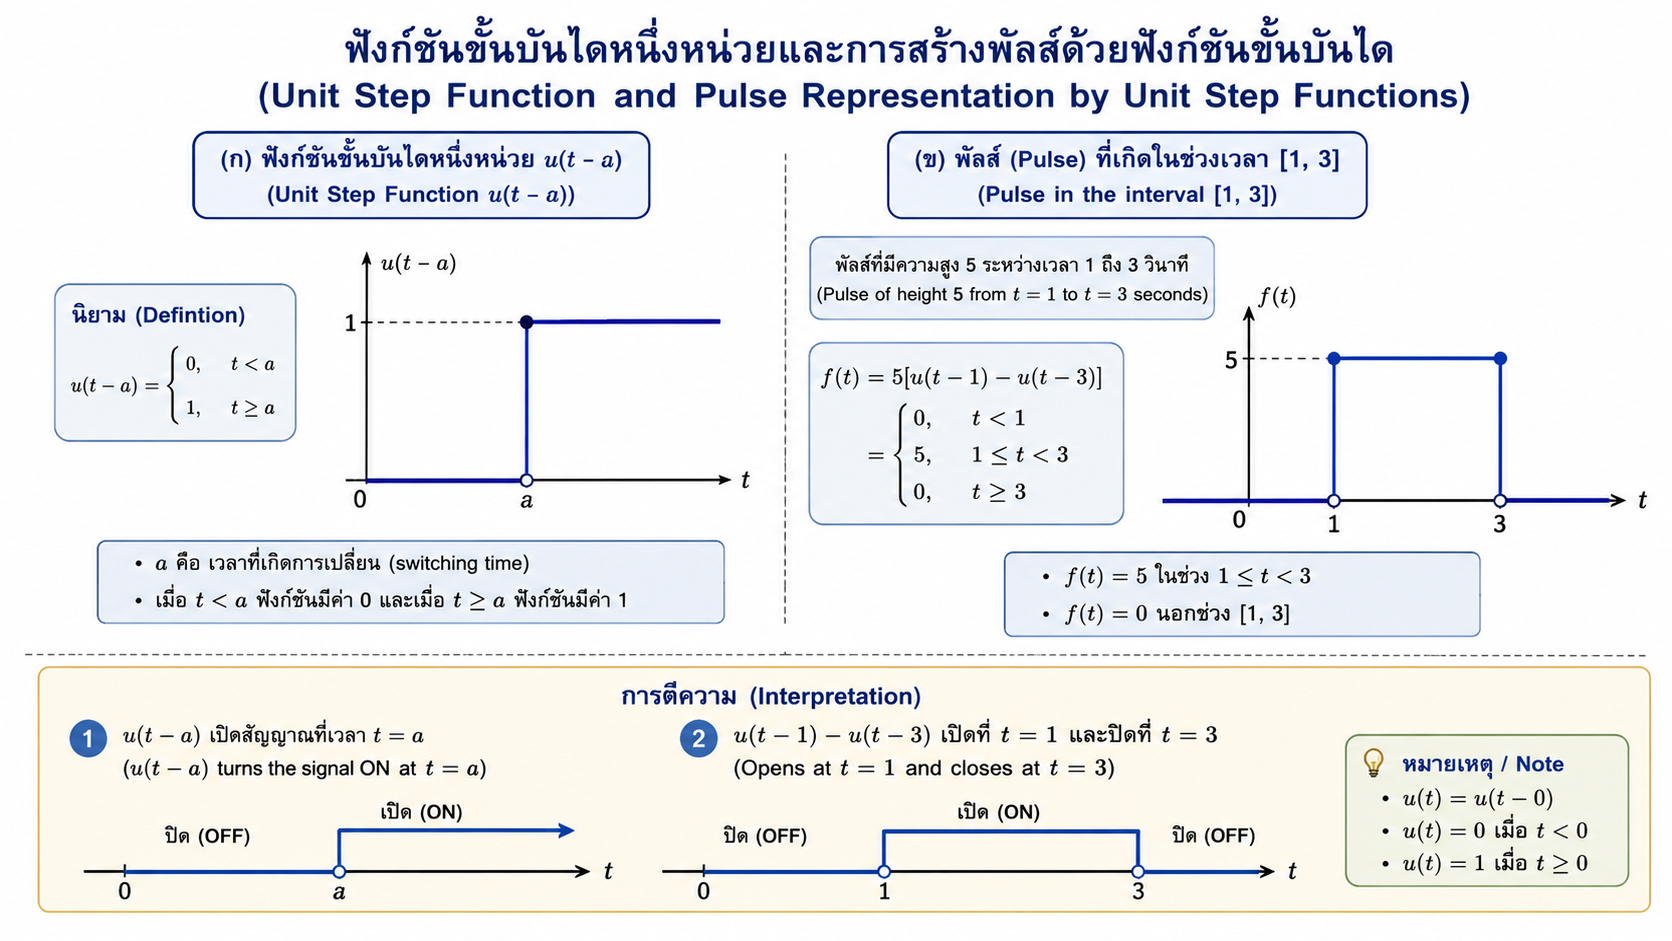
\includegraphics[width=0.8\textwidth]{images/chapter6/figure-04.png}
    \caption{Unit Step และพัลส์สี่เหลี่ยมจากผลต่างของ Unit Step}
\end{figure}

\subsubsection{7.7.4 ตัวอย่างประยุกต์: แรงดันเปิดหลังเวลาหน่วง}

\textbf{ตัวอย่างที่ 6.7 — ตัวอย่างเพิ่มเติมเพื่อการเรียนรู้}\\
แหล่งแรงดันอุดมคติขนาด $12\,\mathrm{V}$ ถูกเปิดที่ $t=0.5\,\mathrm{s}$ จงเขียนสัญญาณและหาลาปลาซ

สัญญาณแรงดันคือ

\[
v(t)=12u(t-0.5)\ \mathrm{V}
\]

จึงได้

\[
V(s)=12\frac{e^{-0.5s}}{s}
\]

\[
\boxed{V(s)=\frac{12e^{-0.5s}}{s}}
\]

หน่วยของ $V(s)$ โดยมิติพื้นฐานเป็น $\mathrm{V\cdot s}$



\subsection{7.8 ฟังก์ชันอิมพัลส์}

\subsubsection{7.8.1 แนวคิดของ Dirac Delta}

ฟังก์ชันอิมพัลส์หนึ่งหน่วย $\delta(t)$ ไม่ใช่ฟังก์ชันธรรมดาในความหมายแบบจุดต่อจุด แต่เป็น generalized function หรือ distribution ที่ใช้แทนเหตุการณ์ที่เกิดในช่วงเวลาสั้นมาก โดยมีคุณสมบัติสำคัญ

\[
\delta(t)=0,\qquad t\ne 0
\]

และ

\[
\boxed{\int_{-\infty}^{\infty}\delta(t)dt=1}
\]

อิมพัลส์ที่เกิดที่เวลา $a$ เขียนเป็น $\delta(t-a)$

\subsubsection{7.8.2 Sampling หรือ Sifting Property}

ถ้า $f(t)$ ต่อเนื่องบริเวณ $t=a$

\[
\boxed{\int_{-\infty}^{\infty}f(t)\delta(t-a)dt=f(a)}
\]

อิมพัลส์จึงทำหน้าที่ “เลือก” ค่าของฟังก์ชัน ณ ตำแหน่งที่อิมพัลส์เกิด

\subsubsection{7.8.3 ลาปลาซของอิมพัลส์}

สำหรับอิมพัลส์หน่วงเวลา $a>0$

\[
\begin{aligned}
    \mathcal{L}\{\delta(t-a)\}&\\
    &=\int_0^{\infty}\delta(t-a)e^{-st}dt\\
    &=e^{-as}
\end{aligned}
\]

ดังนั้น

\[
\boxed{\mathcal{L}\{\delta(t-a)\}=e^{-as}}
\]

และกรณีที่จุดกำเนิดอยู่ภายใต้อนุสัญญาการอินทิเกรตที่รวมอิมพัลส์ไว้

\[
\boxed{\mathcal{L}\{\delta(t)\}=1}
\]

MIT Signals and Systems ใช้ sifting property เพื่อแสดงว่าลาปลาซของ unit impulse มีค่า 1 ภายใต้อนุสัญญาที่ใช้ในการวิเคราะห์สัญญาณ

\subsubsection{7.8.4 ความสัมพันธ์ระหว่าง Unit Step และ Impulse}

ในความหมายของ generalized derivatives

\[
\boxed{\frac{d}{dt}u(t)=\delta(t)}
\]

แนวคิดนี้สำคัญเชิงกายภาพ: step คือการเปลี่ยนระดับแบบฉับพลัน ขณะที่อนุพันธ์ของการเปลี่ยนแบบฉับพลันเป็นอิมพัลส์เชิงอุดมคติ

\subsubsection{7.8.5 ตัวอย่างอิมพัลส์ที่หน่วงเวลา}

\textbf{ตัวอย่างที่ 6.8 — ตัวอย่างพื้นฐาน}\\
จงหาลาปลาซของ

\[
f(t)=4\delta(t-2)
\]

ใช้ linearity และ shifted impulse

\[
F(s)=4e^{-2s}
\]

\[
\boxed{F(s)=4e^{-2s}}
\]

ตัวคูณ 4 คือพื้นที่รวมของอิมพัลส์ และ $e^{-2s}$ บันทึกตำแหน่งเวลา $2\,\mathrm{s}$

% [รูปที่ 5: แนวคิดอิมพัลส์จากพัลส์แคบที่มีพื้นที่คงที่หนึ่งหน่วย]
% ประเภทภาพ: Graph / Infographic
% ตำแหน่งที่แนะนำ: หลังหัวข้อ 7.8.5
% วัตถุประสงค์การเรียนรู้: ช่วยให้ผู้เรียนเข้าใจว่าอิมพัลส์มีความหมายผ่านพื้นที่ ไม่ใช่ “ความสูงอนันต์” เพียงอย่างเดียว
% คำอธิบายภาพ: แสดงพัลส์สี่เหลี่ยมสามรูปที่กว้างลดลง เช่น $\epsilon=1,0.5,0.2$ และสูง $1/\epsilon$ เพื่อให้พื้นที่เท่ากับ 1 ทุกกรณี จากนั้นลูกศรชี้สู่สัญลักษณ์ $\delta(t)$
% องค์ประกอบที่ต้องมี: width $\epsilon$, height $1/\epsilon$, area=1, impulse arrow at t=0
% ข้อความหรือป้ายกำกับ: “พื้นที่คงที่ = 1 / Constant Area = 1”, “narrower”, “higher”, “ideal impulse”
% ภาษาของป้ายกำกับ: ไทยและอังกฤษ
% สัดส่วนภาพ: 16:9
% Image Generation Prompt: Engineering mathematics educational infographic illustrating the Dirac impulse as the limiting idea of rectangular pulses with constant unit area. Show three pulses centered near t=0 with widths epsilon = 1, 0.5, and 0.2 and heights 1/epsilon, each labeled Area = 1, then an arrow toward an ideal impulse delta(t) at t=0. White background, precise axes, bilingual Thai-English labels, vector textbook style, 16:9.
% Graph Generation Prompt: Draw rectangular pulses of width epsilon and height 1/epsilon for epsilon = 1, 0.5, 0.2, each centered at t=0 or starting symmetrically, with annotated area equal to 1. End with a conceptual delta(t) arrow at t=0.
% Alt Text: ภาพแสดงพัลส์สี่เหลี่ยมที่แคบลงและสูงขึ้นโดยรักษาพื้นที่เท่ากับหนึ่ง เพื่ออธิบายแนวคิดเข้าสู่อิมพัลส์อุดมคติที่เวลาเป็นศูนย์

\begin{figure}[htbp]
    \centering
    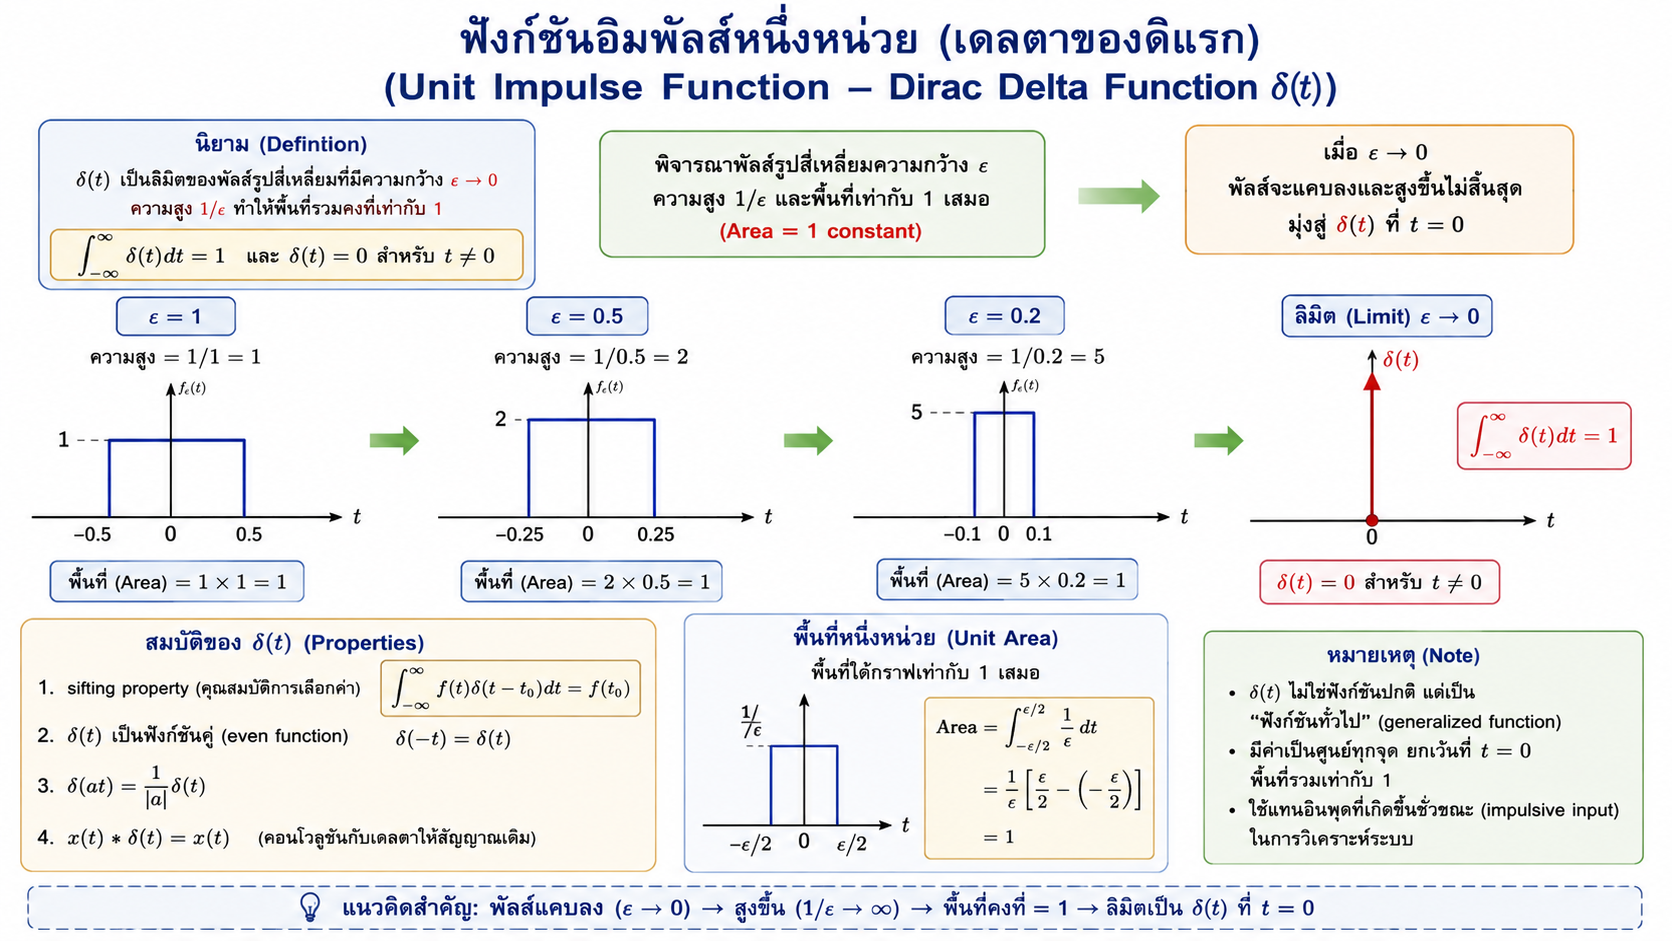
\includegraphics[width=0.8\textwidth]{images/chapter6/figure-05.png}
    \caption{แนวคิดอิมพัลส์จากพัลส์แคบที่มีพื้นที่คงที่หนึ่งหน่วย}
\end{figure}



\subsection{7.9 การแก้สมการเชิงอนุพันธ์ด้วยการแปลงลาปลาซ}

\subsubsection{7.9.1 ขั้นตอนมาตรฐาน}

สำหรับ initial-value problem ควรใช้ขั้นตอนคงที่ดังนี้

\begin{enumerate}
    \item เขียนสมการเชิงอนุพันธ์และเงื่อนไขเริ่มต้นให้ครบ
    \item แปลงลาปลาซทั้งสองข้างของสมการ
    \item แทนสูตรอนุพันธ์โดยใส่เงื่อนไขเริ่มต้นทันที
    \item รวมพจน์ที่มี $Y(s)$
    \item แก้สมการพีชคณิตหา $Y(s)$
    \item จัดรูป $Y(s)$ ให้เทียบตารางได้ เช่น partial fractions หรือ completing the square
    \item หา inverse Laplace เพื่อได้ $y(t)$
    \item ตรวจสอบเงื่อนไขเริ่มต้นและ/หรือแทนกลับในสมการ
    \item ตีความพฤติกรรมของคำตอบ
\end{enumerate}

% [รูปที่ 6: กระบวนการแก้ Initial-Value Problem ด้วยการแปลงลาปลาซ]
% ประเภทภาพ: Flowchart
% ตำแหน่งที่แนะนำ: หลังหัวข้อ 7.9.1
% วัตถุประสงค์การเรียนรู้: ให้ผู้เรียนมีขั้นตอนมาตรฐานเพื่อลดการตกหล่นของเงื่อนไขเริ่มต้น
% คำอธิบายภาพ: ODE + initial conditions → Laplace both sides → substitute derivative rules → solve algebraically for Y(s) → simplify/partial fractions → inverse Laplace → verify initial conditions and ODE → interpret response
% องค์ประกอบที่ต้องมี: กล่อง 8 ขั้น ลูกศรตามลำดับ และกล่องเตือน “ใส่ initial conditions ก่อนจัดรูป”
% ข้อความหรือป้ายกำกับ: ไทยและอังกฤษ
% ภาษาของป้ายกำกับ: ไทยและอังกฤษ
% สัดส่วนภาพ: 16:9
% Image Generation Prompt: Clean engineering mathematics flowchart for solving an initial-value differential equation using the Laplace transform. Steps: ODE plus initial conditions, transform both sides, apply derivative formulas, insert initial conditions, solve algebraically for Y(s), simplify with partial fractions or completing the square, inverse Laplace, verify initial conditions and original ODE, interpret the response. Highlight a warning box: “Do not forget initial conditions.” Bilingual Thai-English labels, white background, vector textbook style, 16:9.
% Alt Text: ผังงานแสดงแปดขั้นตอนในการแก้สมการเชิงอนุพันธ์ด้วยลาปลาซตั้งแต่เขียนเงื่อนไขเริ่มต้นจนตรวจคำตอบ

\begin{figure}[htbp]
    \centering
    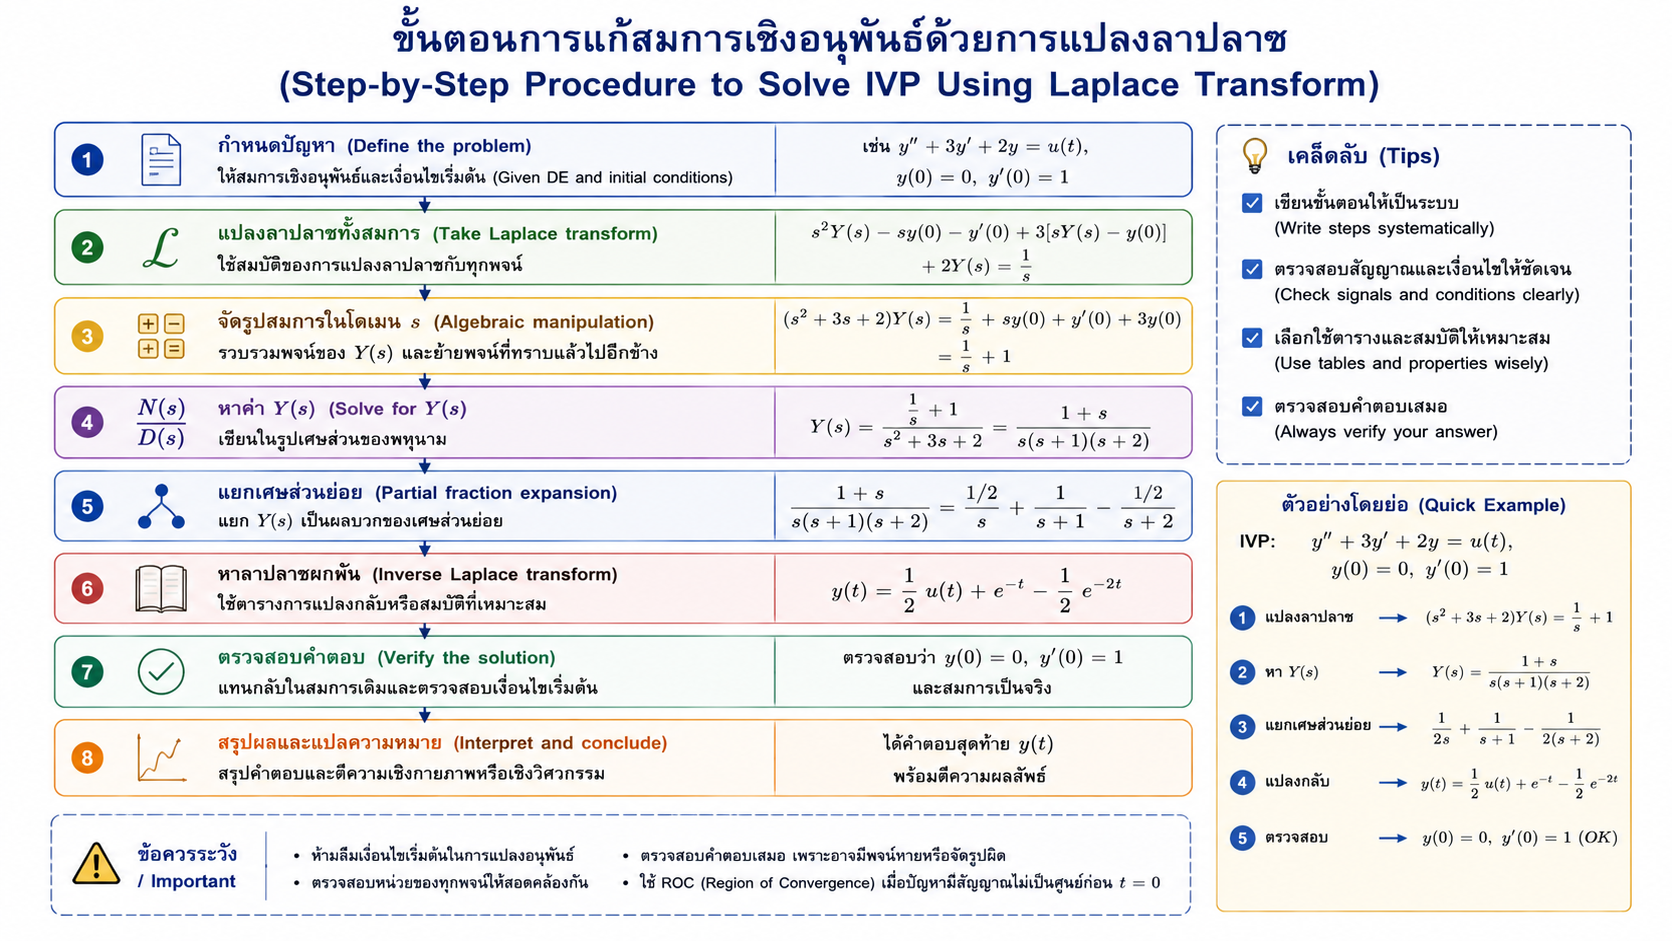
\includegraphics[width=0.8\textwidth]{images/chapter6/figure-06.png}
    \caption{กระบวนการแก้ Initial-Value Problem ด้วยการแปลงลาปลาซ}
\end{figure}

\subsubsection{7.9.2 ตัวอย่างสมการอันดับหนึ่ง}

\textbf{ตัวอย่างที่ 6.9 — ตัวอย่างเชิงวิเคราะห์}\\
จงแก้

\[
y'(t)+2y(t)=6,\qquad y(0)=1
\]

\textbf{1) วิเคราะห์ระบบ} เป็น ODE เชิงเส้นอันดับหนึ่ง มีอินพุตค่าคงที่และมีเงื่อนไขเริ่มต้นหนึ่งค่า

\textbf{2) แปลงลาปลาซทั้งสองข้าง}

\[
\mathcal{L}\{y'\}+2\mathcal{L}\{y\}=6\mathcal{L}\{1\}
\]

ให้ $Y(s)=\mathcal{L}\{y(t)\}$

\[
sY(s)-y(0)+2Y(s)=\frac{6}{s}
\]

แทน $y(0)=1$

\[
(s+2)Y(s)-1=\frac{6}{s}
\]

\textbf{3) แก้หา $Y(s)$}

\[
\begin{aligned}
    Y(s)&=\frac{1+6/s}{s+2}\\
    &=\frac{s+6}{s(s+2)}
\end{aligned}
\]

\textbf{4) แยกเศษส่วนย่อย}

\[
\frac{s+6}{s(s+2)}=\frac{3}{s}-\frac{2}{s+2}
\]

\textbf{5) Inverse Laplace}

\[
\boxed{y(t)=3-2e^{-2t}}
\]

\textbf{6) ตรวจสอบเงื่อนไขเริ่มต้น}

\[
y(0)=3-2=1
\]

ถูกต้อง

\textbf{7) ตรวจสอบค่าสุดท้าย}

\[
\lim_{t\to\infty}y(t)=3
\]

สอดคล้องกับสมการในภาวะคงตัว เพราะถ้า $y'=0$ จะได้ $2y=6$ หรือ $y=3$

\subsubsection{7.9.3 ตัวอย่างสมการอันดับสอง}

\textbf{ตัวอย่างที่ 6.10 — ตัวอย่างเชิงวิเคราะห์}\\
จงแก้

\[
y''(t)+4y(t)=8u(t),\qquad y(0)=0,\quad y'(0)=2
\]

\textbf{1) แปลงลาปลาซ}

\[
s^2Y(s)-sy(0)-y'(0)+4Y(s)=\frac{8}{s}
\]

แทนเงื่อนไขเริ่มต้น

\[
s^2Y(s)-2+4Y(s)=\frac{8}{s}
\]

ดังนั้น

\[
(s^2+4)Y(s)=2+\frac{8}{s}
\]

\[
Y(s)=\frac{2}{s^2+4}+\frac{8}{s(s^2+4)}
\]

\textbf{2) แยกพจน์ที่สอง}

\[
\frac{8}{s(s^2+4)}=\frac{2}{s}-\frac{2s}{s^2+4}
\]

ดังนั้น

\[
Y(s)=\frac{2}{s}-\frac{2s}{s^2+4}+\frac{2}{s^2+4}
\]

\textbf{3) Inverse Laplace}

เนื่องจาก

\[
\mathcal{L}^{-1}\left\{\frac{2}{s^2+4}\right\}=\sin 2t
\]

จึงได้

\[
\boxed{y(t)=2-2\cos 2t+\sin 2t}
\]

\textbf{4) ตรวจสอบค่าเริ่มต้น}

\[
y(0)=2-2+0=0
\]

และ

\[
y'(t)=4\sin 2t+2\cos 2t
\]

ดังนั้น $y'(0)=2$ ถูกต้อง

\subsubsection{7.9.4 ตัวอย่างอินพุตเปิดล่าช้า}

\textbf{ตัวอย่างที่ 6.11 — ตัวอย่างประยุกต์}\\
จงแก้

\[
y'(t)+y(t)=u(t-2),\qquad y(0)=0
\]

แปลงลาปลาซ

\[
sY(s)+Y(s)=\frac{e^{-2s}}{s}
\]

จึงได้

\[
Y(s)=e^{-2s}\frac{1}{s(s+1)}
\]

แยก

\[
\frac{1}{s(s+1)}=\frac{1}{s}-\frac{1}{s+1}
\]

ให้

\[
g(t)=1-e^{-t}
\]

ใช้ time-shift

\[
\boxed{y(t)=u(t-2)\left[1-e^{-(t-2)}\right]}
\]

\textbf{การแปลความหมาย:} ก่อน $t=2$ อินพุตยังไม่เปิด จึงได้ $y(t)=0$ หลัง $t=2$ ระบบเริ่มตอบสนองโดยใช้เวลาใหม่ $t-2$



\subsection{7.10 ความสัมพันธ์ระหว่างลาปลาซกับระบบเชิงเส้น}

\subsubsection{7.10.1 ระบบ LTI และสมการอินพุต–เอาต์พุต}

ระบบเชิงเส้นไม่แปรตามเวลา (LTI) ที่มีสัมประสิทธิ์คงที่อาจเขียนในรูป

\[
a_n\frac{d^ny}{dt^n}+a_{n-1}\frac{d^{n-1}y}{dt^{n-1}}+\cdots+a_0y = b_m\frac{d^mx}{dt^m}+\cdots+b_0x
\]

เมื่อแปลงลาปลาซ สมการอนุพันธ์เปลี่ยนเป็นพหุนามใน $s$ พร้อมพจน์เงื่อนไขเริ่มต้น

ในกรณีเงื่อนไขเริ่มต้นเป็นศูนย์ สามารถเขียนความสัมพันธ์ได้ในรูป

\[
A(s)Y(s)=B(s)X(s)
\]

หรือ

\[
\boxed{Y(s)=G(s)X(s)}
\]

โดย

\[
G(s)=\frac{B(s)}{A(s)}
\]

ในบทนี้ให้มอง $G(s)$ เป็น \textbf{ตัวแทนความสัมพันธ์อินพุต–เอาต์พุตในโดเมน $s$ ภายใต้เงื่อนไขเริ่มต้นเป็นศูนย์} ส่วนการพัฒนาความหมายของฟังก์ชันถ่ายโอน โพล ซีโร และการใช้กับวงจรไฟฟ้าจะอยู่ในบทที่ 7

\subsubsection{7.10.2 คอนโวลูชันและลาปลาซ}

สำหรับฟังก์ชัน $f(t)$ และ $g(t)$ นิยามคอนโวลูชันเป็น

\[
\boxed{(f*g)(t)=\int_0^t f(\tau)g(t-\tau)d\tau}
\]

สมบัติสำคัญคือ

\[
\boxed{\mathcal{L}\{f*g\}=F(s)G(s)}
\]

ดังนั้น การคำนวณคอนโวลูชันในเวลา ซึ่งอาจต้องอินทิเกรตทุกค่า $t$ สามารถเปลี่ยนเป็นการคูณธรรมดาในโดเมน $s$

MIT OpenCourseWare เชื่อม convolution, impulse response และ transfer/system function เข้าด้วยกันโดยตรง ซึ่งเป็นสะพานสำคัญไปสู่การวิเคราะห์ระบบและวงจร

\subsubsection{7.10.3 ตัวอย่างคอนโวลูชันอย่างง่าย}

\textbf{ตัวอย่างที่ 6.12 — ตัวอย่างเพิ่มเติมเพื่อการเรียนรู้}\\
ให้ระบบมี impulse response

\[
h(t)=e^{-2t}u(t)
\]

และอินพุต

\[
x(t)=u(t)
\]

หาเอาต์พุตด้วยลาปลาซและตรวจด้วยคอนโวลูชัน

\textbf{วิธีลาปลาซ}

\[
H(s)=\frac{1}{s+2},\qquad X(s)=\frac{1}{s}
\]

ดังนั้น

\[
\begin{aligned}
    Y(s)&=\frac{1}{s(s+2)}\\
    &=\frac{1/2}{s}-\frac{1/2}{s+2}
\end{aligned}
\]

จึงได้

\[
\boxed{y(t)=\frac{1}{2}\left(1-e^{-2t}\right)u(t)}
\]

\textbf{ตรวจด้วยคอนโวลูชัน}

\[
y(t)=\int_0^t e^{-2(t-\tau)}(1)d\tau
\]

\[
\begin{aligned}
    y(t)&=e^{-2t}\int_0^t e^{2\tau}d\tau\\
    &=\frac{1}{2}(1-e^{-2t})
\end{aligned}
\]

ได้คำตอบตรงกัน

% [รูปที่ 7: ความสัมพันธ์ Input–System–Output ระหว่างโดเมนเวลาและโดเมน s]
% ประเภทภาพ: Block Diagram
% ตำแหน่งที่แนะนำ: หลังหัวข้อ 7.10.3
% วัตถุประสงค์การเรียนรู้: เชื่อม convolution ในเวลากับการคูณในโดเมน s
% คำอธิบายภาพ: แถวบน Time Domain: x(t) → LTI system h(t) → y(t)=x*h. แถวล่าง s-Domain: X(s) → G(s) → Y(s)=G(s)X(s). มีลูกศร Laplace transform เชื่อมแนวตั้งระหว่างคู่ x↔X, h↔G, y↔Y
% องค์ประกอบที่ต้องมี: input block, system block, output block, convolution sign, multiplication sign, transform arrows
% ข้อความหรือป้ายกำกับ: “คอนโวลูชัน / Convolution”, “การคูณ / Multiplication”, “LTI System”
% ภาษาของป้ายกำกับ: ไทยและอังกฤษ
% สัดส่วนภาพ: 16:9
% Image Generation Prompt: Engineering textbook block diagram comparing time domain and s-domain descriptions of an LTI system. Top row: input x(t) enters an LTI system labeled h(t), producing y(t)=x(t)*h(t), emphasizing convolution. Bottom row: X(s) enters G(s), producing Y(s)=G(s)X(s), emphasizing multiplication. Vertical Laplace-transform arrows connect x to X, h to G, and y to Y. White background, bilingual Thai-English labels, precise vector style, 16:9.
% Alt Text: แผนภาพสองแถวแสดงว่าอินพุตคอนโวลูชันกับ impulse response ในโดเมนเวลาสอดคล้องกับการคูณ X(s) และ G(s) ในโดเมน s

\begin{figure}[htbp]
    \centering
    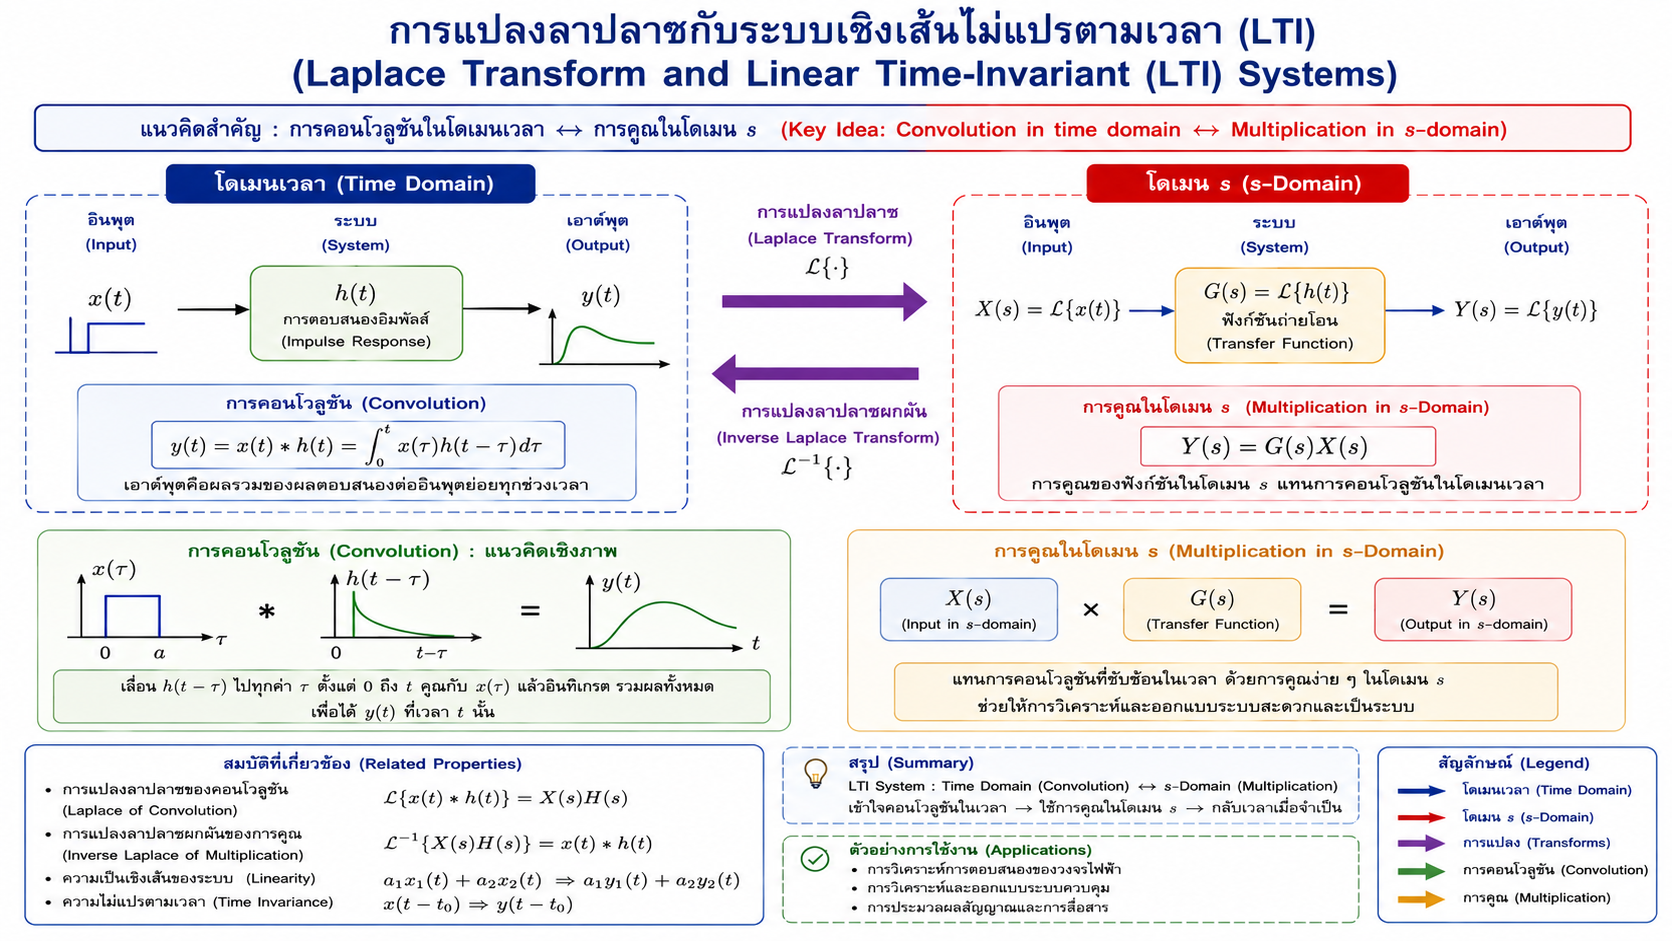
\includegraphics[width=0.8\textwidth]{images/chapter6/figure-07.png}
    \caption{ความสัมพันธ์ Input–System–Output ระหว่างโดเมนเวลาและโดเมน s}
\end{figure}



\subsection{7.11 ตัวอย่างโจทย์และการคำนวณแบบเป็นขั้นตอน}

ส่วนนี้รวบรวมตัวอย่างบูรณาการเพิ่มเติม โดยเน้นกระบวนการคิดตาม Module B: วิเคราะห์โจทย์ กำหนดตัวแปร เลือกหลักการ สร้างและจัดรูปสมการ แปลงโดเมน ตรวจสอบ และแปลความหมาย

\subsubsection{ตัวอย่างที่ 6.13 — Inverse Laplace ที่มีรากจริงต่างกัน}

\textbf{ตัวอย่างเพิ่มเติมเพื่อการเรียนรู้}

จงหา

\[
f(t)=\mathcal{L}^{-1}\left\{\frac{5s+8}{s^2+5s+6}\right\}
\]

\textbf{1) วิเคราะห์ตัวส่วน}

\[
s^2+5s+6=(s+2)(s+3)
\]

\textbf{2) ตั้งเศษส่วนย่อย}

\[
\frac{5s+8}{(s+2)(s+3)}=\frac{A}{s+2}+\frac{B}{s+3}
\]

\textbf{3) หา $A$} แทน $s=-2$

\[
A=\frac{5(-2)+8}{1}=-2
\]

\textbf{4) หา $B$} แทน $s=-3$

\[
B=\frac{5(-3)+8}{-1}=7
\]

ดังนั้น

\[
F(s)=-\frac{2}{s+2}+\frac{7}{s+3}
\]

\textbf{5) Inverse Laplace}

\[
\boxed{f(t)=-2e^{-2t}+7e^{-3t}}
\]

\textbf{6) ตรวจสอบค่าเริ่มต้น}

\[
f(0)=5
\]

และ

\[
\lim_{s\to\infty}sF(s)=5
\]

ตรงกัน

\subsubsection{ตัวอย่างที่ 6.14 — Inverse Laplace ที่ให้การสั่นลดทอน}

\textbf{ตัวอย่างเพิ่มเติมเพื่อการเรียนรู้}

จงหา

\[
\mathcal{L}^{-1}\left\{\frac{6}{s^2+6s+25}\right\}
\]

จัดกำลังสองสมบูรณ์

\[
s^2+6s+25=(s+3)^2+16
\]

ดังนั้น

\[
\begin{aligned}
    F(s)&=\frac{6}{(s+3)^2+4^2}\\
    &=\frac{3}{2}\frac{4}{(s+3)^2+4^2}
\end{aligned}
\]

จึงได้

\[
\boxed{f(t)=\frac{3}{2}e^{-3t}\sin 4t}
\]

\textbf{การแปลความหมาย:} คำตอบเป็นการสั่นด้วยความถี่เชิงมุม $4\,\mathrm{rad/s}$ และแอมพลิจูดถูกครอบด้วยเอกซ์โพเนนเชียล $e^{-3t}$

\subsubsection{ตัวอย่างที่ 6.15 — สัญญาณที่เปิดและปิดหลายช่วง}

\textbf{ตัวอย่างเพิ่มเติมเพื่อการเรียนรู้}

กำหนด

\[
f(t)=
\begin{cases}
0,&0\le t<1\\
3,&1\le t<4\\
1,&t\ge 4
\end{cases}
\]

เขียนด้วย unit step

ที่ $t=1$ สัญญาณเพิ่มจาก 0 เป็น 3 จึงมี $+3u(t-1)$\\
ที่ $t=4$ สัญญาณลดจาก 3 เป็น 1 คือเปลี่ยน $-2$ จึงมี $-2u(t-4)$

ดังนั้น

\[
\boxed{f(t)=3u(t-1)-2u(t-4)}
\]

ลาปลาซคือ

\[
\boxed{F(s)=\frac{3e^{-s}-2e^{-4s}}{s}}
\]

\textbf{ตรวจสอบเชิงช่วงเวลา:}

\begin{itemize}
    \item $t<1$: ทั้งสอง step เป็นศูนย์ $\to f=0$
    \item $1\le t<4$: step แรกเป็น 1 $\to f=3$
    \item $t\ge4$: ทั้งสองเป็น 1 $\to f=3-2=1$
\end{itemize}

\subsubsection{ตัวอย่างที่ 6.16 — ODE ที่มีพัลส์ช่วงจำกัด}

\textbf{ตัวอย่างเพิ่มเติมเพื่อการเรียนรู้}

ให้

\[
y'(t)+2y(t)=10[u(t)-u(t-1)],\qquad y(0)=0
\]

อินพุตขนาด 10 ทำงานตั้งแต่ $0$ ถึง $1\,\mathrm{s}$

แปลงลาปลาซ

\[
(s+2)Y(s)=\frac{10}{s}(1-e^{-s})
\]

ดังนั้น

\[
Y(s)=10(1-e^{-s})\frac{1}{s(s+2)}
\]

แยก

\[
\frac{10}{s(s+2)}=\frac{5}{s}-\frac{5}{s+2}
\]

กำหนด

\[
g(t)=5(1-e^{-2t})
\]

จึงได้

\[
\boxed{y(t)=g(t)-u(t-1)g(t-1)}
\]

หรือ

\[
\boxed{y(t)=5(1-e^{-2t})-5u(t-1)\left[1-e^{-2(t-1)}\right]}
\]

\textbf{แปลความหมาย:} ช่วงแรกระบบสะสมการตอบสนองจากอินพุต 10 เมื่ออินพุตถูกปิดที่ 1 วินาที ส่วนที่สองจะลบ “การตอบสนองที่เกิดจากการเปิดต่อเนื่องหลัง 1 วินาที” ออก ทำให้ได้การตอบสนองต่อพัลส์ช่วงจำกัดอย่างถูกต้อง



\subsection{7.12 กิจกรรมการเรียนรู้และแบบฝึกหัดท้ายบท}

หัวข้อบังคับของรายวิชากำหนดให้มี “กิจกรรมการเรียนรู้และแบบฝึกหัดท้ายบท” ในบทนี้ โดยเนื่องจากไม่ได้เปิดใช้ Module C แบบเต็ม จึงออกแบบกิจกรรมให้กระชับและใช้เพื่อเสริมเนื้อหาหลัก ส่วนแบบฝึกหัดฉบับเต็มอยู่ในหัวข้อ 12

\subsubsection{\texorpdfstring{กิจกรรมสั้นที่ 1: จับคู่ Time Domain กับ $s$-Domain}{กิจกรรมสั้นที่ 1: จับคู่ Time Domain กับ s-Domain}}

ผู้สอนเตรียมบัตร 12 ใบ แบ่งเป็นฟังก์ชันเวลา 6 ใบและฟังก์ชันลาปลาซ 6 ใบ เช่น $1$, $t$, $e^{-2t}$, $\sin 3t$, $u(t-2)$, $\delta(t-1)$ ให้ผู้เรียนจับคู่และอธิบาย “สัญญาณบอกใบ้” ของแต่ละคู่ เช่น ตัวประกอบ $e^{-2s}$ หมายถึงการหน่วงเวลา

\textbf{เป้าหมาย:} CLO6.2 และ CLO6.4\\
\textbf{เวลาที่แนะนำ:} 10–15 นาที\\
\textbf{ประเมิน:} ความถูกต้องของคู่และเหตุผลสั้น ๆ

\subsubsection{กิจกรรมสั้นที่ 2: Error Analysis — ผิดตรงไหน}

ให้ผู้เรียนพิจารณาคำตอบสมมติ

\[
\mathcal{L}\{y''\}=s^2Y(s)-y(0)-y'(0)
\]

แล้วชี้ว่าผิดตรงไหน คำตอบที่ถูกต้องคือ

\[
\mathcal{L}\{y''\}=s^2Y(s)-sy(0)-y'(0)
\]

จากนั้นให้ผู้เรียนสร้าง “รายการตรวจสอบ 3 จุด” ก่อนแก้ ODE ด้วยลาปลาซ

\textbf{เป้าหมาย:} CLO6.5\\
\textbf{เวลาที่แนะนำ:} 10 นาที\\
\textbf{ประเมิน:} คำอธิบายเหตุผล ไม่ใช่เพียงแก้สูตรให้ถูก



\subsection{8. ความเข้าใจผิดที่พบบ่อย}

\subsubsection{\texorpdfstring{8.1 คิดว่า $s$ คือความถี่ $\omega$ โดยตรง}{8.1 คิดว่า s คือความถี่ omega โดยตรง}}

\textbf{ความเข้าใจที่คลาดเคลื่อน:} $s$ กับ $j\omega$ เป็นสิ่งเดียวกันเสมอ\\
\textbf{แนวคิดที่ถูกต้อง:} $s=\sigma+j\omega$ เป็นตัวแปรเชิงซ้อนทั่วไป การแทน $s=j\omega$ เป็นกรณีเฉพาะที่ต้องมีเงื่อนไขเหมาะสมและมักเกิดในการเชื่อมกับการตอบสนองเชิงความถี่

\subsubsection{8.2 ลืมเงื่อนไขเริ่มต้นเมื่อแปลงอนุพันธ์}

ผิด:

\[
\mathcal{L}\{y'\}=sY
\]

ใน initial-value problem ทั่วไป

ถูก:

\[
\mathcal{L}\{y'\}=sY-y(0)
\]

หากเงื่อนไขเริ่มต้นเป็นศูนย์จึงลดรูปเหลือ $sY$

\subsubsection{\texorpdfstring{8.3 ใช้ Time Shift แต่ไม่เปลี่ยนตัวแปรภายในเป็น $t-a$}{8.3 ใช้ Time Shift แต่ไม่เปลี่ยนตัวแปรภายในเป็น t-a}}

ผู้เรียนมักเห็น $u(t-a)f(t)$ แล้วเขียน $e^{-as}F(s)$ ทันที ซึ่งไม่ถูกต้องเสมอ ต้องจัดฟังก์ชันให้อยู่ในรูป

\[
u(t-a)g(t-a)
\]

ก่อน แล้วจึงใช้ $e^{-as}G(s)$

\subsubsection{8.4 แยกเศษส่วนย่อยรากซ้ำไม่ครบกำลัง}

ถ้ามี $(s+1)^2$ ต้องมีทั้ง

\[
\frac{A}{s+1}+\frac{B}{(s+1)^2}
\]

ห้ามเขียนเพียงพจน์เดียว

\subsubsection{8.5 ไม่หารพหุนามก่อนเมื่อดีกรีตัวเศษสูง}

Partial fractions มาตรฐานใช้กับ proper rational function จึงต้องตรวจดีกรีก่อนทุกครั้ง

\subsubsection{\texorpdfstring{8.6 คิดว่า $\delta(t)$ เป็นพัลส์ที่มี “ค่าอนันต์” แบบตัวเลขธรรมดา}{8.6 คิดว่า delta(t) เป็นพัลส์ที่มี ค่าอนันต์ แบบตัวเลขธรรมดา}}

จุดสำคัญของ $\delta(t)$ คือคุณสมบัติผ่านอินทิกรัลและพื้นที่ ไม่ควรจัดการเหมือนฟังก์ชันค่าจริงธรรมดาที่ $t=0$

\subsubsection{8.7 ใช้ Final Value Theorem โดยไม่ตรวจว่าค่าสุดท้ายมีอยู่}

หากคำตอบสั่นต่อเนื่องหรือไม่ลู่เข้า การคำนวณ $\lim_{s\to0}sF(s)$ แบบกลไกอาจให้ข้อสรุปที่ผิด

\subsubsection{\texorpdfstring{8.8 ได้ $Y(s)$ แล้วหยุด}{8.8 ได้ Y(s) แล้วหยุด}}

ในการแก้ปัญหาโดเมนเวลา $Y(s)$ เป็นขั้นกลาง ต้อง inverse Laplace และตรวจเงื่อนไขเริ่มต้นจึงถือว่าคำตอบสมบูรณ์

\subsubsection{ตารางที่ 6.4 สรุปความผิดพลาดและวิธีป้องกัน}

\begin{table}[htbp]
    \centering
    \begin{tabular}{l l l}
        \hline
        \textbf{จุดผิดพลาด} & \textbf{อาการ} & \textbf{วิธีป้องกัน} \\
        \hline
        ลืม initial conditions & ได้สัมประสิทธิ์คำตอบผิด & เขียนสูตร derivative transform ก่อนแทนค่า \\
        time shift ผิด & เวลาเริ่มของคำตอบไม่ตรง & จัดเป็น $u(t-a)g(t-a)$ \\
        partial fraction ไม่ครบ & inverse ไม่สมบูรณ์ & ตรวจชนิดและกำลังของ factor ทุกตัว \\
        quadratic ไม่ complete square & เทียบ sin/cos ไม่ได้ & ทำกำลังสองสมบูรณ์ก่อน \\
        sign error ใน $s$-shift & ได้ growing/decaying สลับกัน & จำ $e^{at}f(t)\leftrightarrow F(s-a)$ \\
        impulse จัดการเหมือนพัลส์ธรรมดา & สับสนหน่วย/พื้นที่ & ใช้ sifting property เป็นหลัก \\
        \hline
    \end{tabular}
\end{table}



\subsection{9. การประยุกต์ใช้ในงานจริง}

\subsubsection{9.1 การวิเคราะห์การเปิด-ปิดสวิตช์ในวงจร}

การเปิดแหล่งจ่าย ณ เวลา $t=a$ สามารถแทนด้วย $V_0u(t-a)$ การเปิดเป็นช่วงเวลาจำกัดแทนด้วยผลต่างของ unit step วิธีนี้ทำให้สัญญาณที่เดิมต้องเขียนแบบหลายช่วงสามารถรวมเป็นสมการเดียวและแปลงลาปลาซได้

\subsubsection{9.2 การจัดการพลังงานสะสมเริ่มต้น}

ตัวเก็บประจุและตัวเหนี่ยวนำอาจมีสถานะเริ่มต้นก่อนสวิตช์ ในบทที่ 7 เงื่อนไขเหล่านี้จะปรากฏผ่าน derivative rules ของลาปลาซ ทำให้ไม่ต้องทิ้งข้อมูลเริ่มต้นขณะเปลี่ยนโดเมน

\subsubsection{9.3 การวิเคราะห์ระบบควบคุมเชิงเส้น}

สมการเชิงอนุพันธ์ของระบบควบคุมสามารถเปลี่ยนเป็นความสัมพันธ์พีชคณิตระหว่าง $X(s)$ และ $Y(s)$ เมื่อกำหนดเงื่อนไขเริ่มต้นเหมาะสม แนวคิดนี้เป็นฐานของ transfer function และ block diagram ในวิชาระบบควบคุม

\subsubsection{9.4 การวิเคราะห์สัญญาณกระตุ้นแบบอิมพัลส์}

Impulse response เป็นแนวคิดสำคัญมาก เพราะสำหรับระบบ LTI เมื่อทราบการตอบสนองต่ออิมพัลส์แล้ว สามารถสร้างการตอบสนองต่ออินพุตทั่วไปผ่าน convolution ได้

\subsubsection{9.5 การเชื่อม Fourier กับ Laplace}

จากบทก่อนหน้า ผู้เรียนคุ้นเคยกับแนวคิดความถี่จาก Fourier series แล้ว Laplace transform ขยายกรอบการมองไปยังตัวแปรเชิงซ้อน $s=\sigma+j\omega$ ทำให้สามารถอธิบายทั้งพฤติกรรมการเพิ่ม/ลดแบบเอกซ์โพเนนเชียลและการสั่นในตัวแทนเดียวกัน

\subsubsection{ตารางที่ 6.5 ตัวอย่างสถานการณ์ทางวิศวกรรมและเครื่องมือในบท}

\begin{table}[htbp]
    \centering
    \small
    \begin{tabularx}{\textwidth}{>{\raggedright\arraybackslash}p{0.30\textwidth} >{\raggedright\arraybackslash}p{0.28\textwidth} X}
        \hline
        \textbf{สถานการณ์} & \textbf{การแทนทางคณิตศาสตร์} & \textbf{เครื่องมือ Laplace ที่ใช้} \\
        \hline
        เปิดแหล่งจ่ายที่ $t=a$ & $V_0u(t-a)$ & time shift \\
        พัลส์แรงดันช่วงสั้น & $V_0[u(t-a)-u(t-b)]$ & step decomposition \\
        แรงกระแทก/สัญญาณกระตุ้นสั้นมาก & $A\delta(t-a)$ & impulse transform \\
        ระบบอันดับหนึ่ง & ODE อันดับหนึ่ง & derivative transform + partial fractions \\
        ระบบอันดับสอง & ODE อันดับสอง & derivative transform + completing square \\
        ระบบ LTI & $y=x*h$ & convolution theorem \\
        \hline
    \end{tabularx}
\end{table}



\subsection{10. สรุปท้ายบท}

\begin{enumerate}
    \item การแปลงลาปลาซเปลี่ยน $f(t)$ ในโดเมนเวลาเป็น $F(s)$ ในโดเมนเชิงซ้อน
\end{enumerate}

\[
F(s)=\int_0^\infty f(t)e^{-st}dt
\]

\begin{enumerate}
    \item การลู่เข้าของอินทิกรัลมีความสำคัญ และสามารถอธิบายด้วยแนวคิด Region of Convergence
    \item ตารางคู่การแปลงช่วยลดภาระการอินทิเกรต แต่ต้องเข้าใจครอบครัวของรูปแบบ เช่น polynomial, exponential และ sinusoidal
    \item สมบัติเชิงเส้นช่วยแยกปัญหาเป็นพจน์ย่อย
    \item การคูณด้วย $e^{at}$ ในเวลาเชื่อมกับการเลื่อน $s$ และการหน่วงเวลาด้วย unit step เชื่อมกับตัวคูณ $e^{-as}$
    \item อนุพันธ์ในเวลาแปลงเป็นพจน์พีชคณิตของ $s$ พร้อมเงื่อนไขเริ่มต้น
\end{enumerate}

\[
\mathcal{L}\{f'\}=sF-f(0)
\]

\[
\mathcal{L}\{f''\}=s^2F-sf(0)-f'(0)
\]

\begin{enumerate}
    \item Inverse Laplace ในงานวิศวกรรมระดับต้นทำได้ด้วย table lookup, completing the square และ partial fractions
    \item Unit step ใช้แทนการเปิด/ปิดอินพุตตามเวลา ส่วน impulse ใช้แทนอินพุตเชิงอุดมคติที่มีพื้นที่จำกัดและช่วงเวลาสั้นมาก
    \item วิธีแก้ ODE ด้วยลาปลาซคือ แปลง $\to$ ใส่ initial conditions $\to$ แก้ $Y(s)$ $\to$ จัดรูป $\to$ inverse $\to$ ตรวจคำตอบ
    \item Convolution ในเวลาเปลี่ยนเป็นการคูณในโดเมน $s$
\end{enumerate}

\[
\mathcal{L}\{f*g\}=F(s)G(s)
\]

\begin{enumerate}
    \item ความสัมพันธ์ $Y(s)=G(s)X(s)$ ภายใต้เงื่อนไขเริ่มต้นเป็นศูนย์เป็นสะพานไปสู่บทที่ 7 เรื่องการวิเคราะห์วงจรและฟังก์ชันถ่ายโอน
    \item จุดที่ต้องระวังคืออนุสัญญาค่า ณ $t=0$, การเขียน time shift ให้ถูก และเงื่อนไขของทฤษฎีค่าสุดท้าย
\end{enumerate}



\subsection{11. คำถามทบทวน}

\begin{enumerate}
    \item เพราะเหตุใดการแปลงลาปลาซจึงช่วยให้การแก้สมการเชิงอนุพันธ์เชิงเส้นง่ายขึ้นในหลายกรณี
    \item ตัวแปร $s=\sigma+j\omega$ แตกต่างจากความถี่เชิงมุม $\omega$ อย่างไร
    \item Region of Convergence มีความหมายอย่างไร และเหตุใดนิพจน์ $F(s)$ เพียงอย่างเดียวอาจไม่บอกข้อมูลทั้งหมดของการแปลง
    \item อธิบายความแตกต่างระหว่าง $s$-shifting กับ time shifting พร้อมยกตัวอย่างคนละหนึ่งกรณี
    \item เหตุใด $\mathcal{L}\{y'\}$ จึงมีพจน์เงื่อนไขเริ่มต้น และผลนี้มีประโยชน์ต่อวิศวกรรมอย่างไร
    \item เมื่อใดควรใช้ partial fractions และต้องตรวจอะไรกับดีกรีของตัวเศษและตัวส่วนก่อน
    \item Unit step และ impulse มีบทบาทต่างกันอย่างไรในการแทนเหตุการณ์สวิตชิง
    \item อธิบายความหมายของสัญลักษณ์ $e^{-as}$ ที่พบใน $F(s)$ ในมุมมองของการหน่วงเวลา
    \item เพราะเหตุใด convolution ในโดเมนเวลาจึงมีความสัมพันธ์สำคัญกับระบบ LTI
    \item ให้เหตุผลว่าทำไมการใช้ Final Value Theorem จึงต้องตรวจเงื่อนไขก่อนเสมอ
\end{enumerate}

\newpage

\subsection{12. แบบฝึกหัดท้ายบท}

แบบฝึกหัดจัดตาม Module E จากง่ายไปยากเป็น 3 ระดับ ได้แก่ \textbf{พื้นฐาน 5 ข้อ วิเคราะห์ 5 ข้อ และประยุกต์ใช้ 3 ข้อ} เฉลยละเอียดอยู่ในภาคผนวกสำหรับผู้สอนท้ายเอกสาร

\subsubsection{12.1 ระดับพื้นฐาน}

\paragraph{ข้อ 1}

จงหา Laplace transform ของ

\[
f(t)=4+2t+3t^2
\]

\paragraph{ข้อ 2}

จงหา Laplace transform ของ

\[
f(t)=5e^{-2t}-4\sin 3t+2\cos 3t
\]

\paragraph{ข้อ 3}

จงหา inverse Laplace ของ

\[
F(s)=\frac{6}{s}+\frac{2}{s+4}-\frac{3}{s^2}
\]

\paragraph{ข้อ 4}

จงหา Laplace transform ของ

\[
f(t)=u(t-3)
\]

และอธิบายความหมายของตัวประกอบที่เกิดจากการหน่วงเวลา

\paragraph{ข้อ 5}

จงหา Laplace transform ของ

\[
f(t)=7\delta(t-0.5)
\]

และระบุความหมายของเลข 7 ในมุมมองพื้นที่ของอิมพัลส์

\subsubsection{12.2 ระดับวิเคราะห์}

\paragraph{ข้อ 6}

จงหา inverse Laplace โดยใช้ partial fractions

\[
F(s)=\frac{4s+9}{(s+1)(s+2)}
\]

\paragraph{ข้อ 7}

จงหา inverse Laplace

\[
F(s)=\frac{2s+5}{s(s+2)^2}
\]

\paragraph{ข้อ 8}

จงหา inverse Laplace

\[
F(s)=\frac{3s+12}{s^2+4s+13}
\]

พร้อมอธิบายว่าคำตอบมีลักษณะลดทอนหรือไม่

\paragraph{ข้อ 9}

ใช้การแปลงลาปลาซแก้

\[
y'(t)+3y(t)=9,\qquad y(0)=2
\]

และตรวจสอบค่าสุดท้ายด้วยสมการเดิม

\paragraph{ข้อ 10}

ใช้การแปลงลาปลาซแก้

\[
\begin{aligned}
    y''(t)+5y'(t)+6y(t)&=0,\\
    \qquad y(0)&=1,\quad y'(0)=0
\end{aligned}
\]

\subsubsection{12.3 ระดับประยุกต์ใช้}

\paragraph{ข้อ 11}

ระบบอันดับหนึ่งถูกกระตุ้นด้วยอินพุตที่เริ่มที่ $t=2\,\mathrm{s}$

\[
y'(t)+2y(t)=8u(t-2),\qquad y(0)=0
\]

จงหา $y(t)$ และอธิบายพฤติกรรมก่อนและหลัง $t=2\,\mathrm{s}$

\paragraph{ข้อ 12}

ให้

\[
y'(t)+y(t)=5[u(t)-u(t-3)],\qquad y(0)=0
\]

จงหา $y(t)$ และอธิบายว่าการปิดอินพุตที่ $t=3\,\mathrm{s}$ ปรากฏในคำตอบอย่างไร

\paragraph{ข้อ 13}

ระบบ LTI มี impulse response

\[
h(t)=e^{-3t}u(t)
\]

และอินพุตเป็นพัลส์

\[
x(t)=u(t)-u(t-2)
\]

จงหา $Y(s)$ และ $y(t)$ โดยใช้สมบัติลาปลาซ พร้อมอธิบายความสัมพันธ์กับ convolution

\newpage

\subsection{13. ข้อเสนอแนะสำหรับผู้สอน}

\subsubsection{13.1 ลำดับการสอนที่แนะนำสำหรับ 2 สัปดาห์}

\textbf{สัปดาห์ที่ 11}

\begin{itemize}
    \item 20 นาที: Motivation จาก ODE ในงานไฟฟ้าและแนวคิด time domain $\to$ $s$-domain
    \item 35 นาที: นิยาม การลู่เข้า และคู่การแปลงจากนิยาม 2 ตัวอย่าง
    \item 35 นาที: ตารางพื้นฐานและสมบัติเชิงเส้น/$s$-shift
    \item 40 นาที: derivative rules และการใช้ initial conditions
    \item 30 นาที: inverse Laplace และ partial fractions
    \item 20 นาที: แบบฝึกหัดร่วมกันและ formative assessment
\end{itemize}

\textbf{สัปดาห์ที่ 12}

\begin{itemize}
    \item 25 นาที: ทบทวน inverse Laplace และ partial fractions
    \item 35 นาที: unit step และ time shift
    \item 25 นาที: impulse และ sifting property
    \item 55 นาที: แก้ ODE อันดับหนึ่งและอันดับสองแบบเป็นขั้นตอน
    \item 25 นาที: delayed input / pulse input
    \item 20 นาที: ความสัมพันธ์กับ LTI และ convolution
    \item 15 นาที: exit ticket เชื่อมไปบทที่ 7
\end{itemize}

\subsubsection{13.2 จุดที่ผู้เรียนมักมีปัญหา}

\begin{enumerate}
    \item สลับเครื่องหมายใน $s$-shifting เช่น $e^{-at}$ ต้องสัมพันธ์กับ $F(s+a)$
    \item ลืม $s$ ที่คูณ initial condition ในอนุพันธ์อันดับสอง
    \item ตั้ง partial fractions สำหรับรากซ้ำไม่ครบ
    \item ไม่ complete square ก่อนเทียบไซน์/โคไซน์
    \item ใช้ time shift โดยไม่ได้เขียนฟังก์ชันภายในเป็น $t-a$
    \item ไม่แยกความแตกต่างระหว่าง step และ impulse
    \item จำสูตรโดยไม่ตรวจค่าสุดท้ายหรือค่าเริ่มต้น ทำให้ไม่พบความผิดพลาดเชิงพีชคณิต
\end{enumerate}

\subsubsection{13.3 วิธีเลือกตัวอย่าง}

ควรเลือกตัวอย่างที่ทำให้ “เหตุผลในการใช้ลาปลาซ” เห็นชัด ได้แก่

\begin{itemize}
    \item ODE ที่มี initial conditions ไม่เป็นศูนย์
    \item สัญญาณที่เปิดหลังเวลาหน่วง
    \item พัลส์ที่เปิดและปิด
    \item ODE ที่ตัวส่วนหลังแปลงมีทั้งรากจริงและรากเชิงซ้อน
\end{itemize}

หลีกเลี่ยงการเริ่มด้วยโจทย์เศษส่วนย่อยที่ยาวมาก เพราะผู้เรียนอาจเข้าใจผิดว่าลาปลาซเป็นเพียงเทคนิคพีชคณิตที่ซับซ้อน

\subsubsection{13.4 การประเมินระหว่างเรียน}

ใช้ exit ticket 3 ข้อ เช่น

\begin{enumerate}
    \item เขียน $\mathcal{L}\{y''\}$ พร้อม initial conditions
    \item เขียน $3u(t-2)$ ในโดเมน $s$
    \item ระบุวิธีแรกที่ควรทำกับ $F(s)=(2s+1)/(s^2+4s+8)$ ก่อน inverse Laplace
\end{enumerate}

หากผู้เรียนตอบข้อ 1 ผิด ควรทบทวน derivative rule ก่อนเริ่ม ODE เพิ่มเติม หากข้อ 2 ผิด ให้ทบทวน time shift และหากข้อ 3 ผิด ให้ทบทวน completing the square

\subsubsection{13.5 แนวทางการตรวจคำตอบ}

ให้คะแนนไม่เพียงคำตอบสุดท้าย แต่พิจารณา

\begin{itemize}
    \item การตั้ง $Y(s)$ ถูกต้อง
    \item การใส่เงื่อนไขเริ่มต้นถูกตำแหน่ง
    \item การเลือกวิธีจัดรูปเหมาะสม
    \item partial fractions ถูกต้อง
    \item inverse Laplace ถูกคู่
    \item ตรวจสอบค่าเริ่มต้นหรือพฤติกรรมค่าสุดท้าย
\end{itemize}

สิ่งนี้ช่วยให้การประเมินสอดคล้องกับ CLO6.3–CLO6.5 มากกว่าการวัดเพียงทักษะพีชคณิต



\subsection{14. สื่อและแหล่งเรียนรู้เพิ่มเติม}

รายการนี้จัดตาม Module H โดยแยก “สื่อแนะนำ” ออกจาก “เอกสารอ้างอิงทางวิชาการ” และใช้เฉพาะแหล่งที่ตรวจสอบพบจริง

\subsubsection{14.1 MIT OpenCourseWare — Differential Equations}

\begin{itemize}
    \item \textbf{องค์กร/ผู้จัดทำ:} Massachusetts Institute of Technology, MIT OpenCourseWare
    \item \textbf{หัวข้อที่ควรค้น:} Laplace Transform: Basics; Partial Fractions and Inverse Laplace Transform; Laplace Transform: Solving Initial Value Problems; Step and Delta; Convolution
    \item \textbf{คำค้นแนะนำ:} \texttt{MIT OCW 18.03SC Laplace Transform Basics}, \texttt{MIT OCW partial fractions inverse Laplace}, \texttt{MIT OCW solving initial value problems Laplace}
    \item \textbf{จุดประสงค์ในการรับชม:} เสริมภาพรวม แนวคิดการแปลง ODE เป็นสมการพีชคณิต วิธี inverse Laplace และการใช้ step/delta
    \item \textbf{ช่วงเวลาที่เหมาะสม:} หลังสอน 7.4–7.9 หรือมอบหมายก่อนชั้นเรียนสัปดาห์ที่ 12
\end{itemize}

\subsubsection{14.2 MIT OpenCourseWare — Signals and Systems}

\begin{itemize}
    \item \textbf{องค์กร/ผู้จัดทำ:} Massachusetts Institute of Technology, MIT OpenCourseWare
    \item \textbf{หัวข้อที่ควรค้น:} Lecture 6: Laplace Transform
    \item \textbf{คำค้นแนะนำ:} \texttt{MIT 6.003 Laplace transform lecture 6}
    \item \textbf{จุดประสงค์ในการรับชม:} เชื่อม Laplace transform กับ signals, systems, derivative property และ impulse
    \item \textbf{ช่วงเวลาที่เหมาะสม:} หลังหัวข้อ 7.8 และ 7.10
\end{itemize}

\subsubsection{14.3 NIST Digital Library of Mathematical Functions (DLMF)}

\begin{itemize}
    \item \textbf{องค์กร/ผู้จัดทำ:} National Institute of Standards and Technology (NIST)
    \item \textbf{หัวข้อที่ควรค้น:} Section 1.14 Integral Transforms — Laplace Transform
    \item \textbf{คำค้นแนะนำ:} \texttt{NIST DLMF 1.14 Laplace transform}
    \item \textbf{จุดประสงค์ในการใช้:} ตรวจสอบนิยาม เงื่อนไขการลู่เข้า shifting derivative property periodic functions และ convolution theorem
    \item \textbf{ช่วงเวลาที่เหมาะสม:} ใช้เป็นแหล่งอ้างอิงสำหรับผู้สอนหรือผู้เรียนที่ต้องการความแม่นยำเชิงนิยาม
\end{itemize}

\subsubsection{14.4 Cambridge University Press — A Student's Guide to Laplace Transforms}

\begin{itemize}
    \item \textbf{ผู้จัดทำ:} Daniel Fleisch
    \item \textbf{หัวข้อที่ควรค้น:} Laplace-transform examples, properties, applications
    \item \textbf{คำค้นแนะนำ:} \texttt{Daniel Fleisch Student's Guide to Laplace Transforms Cambridge}
    \item \textbf{จุดประสงค์ในการใช้:} เสริม intuition ของคู่การแปลงและการประยุกต์ทางฟิสิกส์/วิศวกรรม
    \item \textbf{ช่วงเวลาที่เหมาะสม:} ใช้อ่านเสริมหลังเรียนพื้นฐานหรือสำหรับนักศึกษาที่ต้องการคำอธิบายเชิงความหมายมากขึ้น
\end{itemize}

\subsubsection{14.5 Wiley — Advanced Engineering Mathematics}

\begin{itemize}
    \item \textbf{ผู้จัดทำ:} Erwin Kreyszig
    \item \textbf{หัวข้อที่ควรค้น:} Chapter 6 Laplace Transforms; Linearity; Shifting; Transforms of Derivatives and Integrals; ODEs
    \item \textbf{คำค้นแนะนำ:} \texttt{Wiley Kreyszig Advanced Engineering Mathematics Laplace Transforms}
    \item \textbf{จุดประสงค์ในการใช้:} แบบฝึกหัดและการจัดลำดับเนื้อหาวิศวกรรมคณิตศาสตร์มาตรฐาน
    \item \textbf{ช่วงเวลาที่เหมาะสม:} ใช้เป็นตำราหลักหรืออ่านเสริมตลอดบท
\end{itemize}

\newpage

\subsection{15. เอกสารอ้างอิง}

\begin{quote}
\textbf{รูปแบบ:} APA 7
รายการอ้างอิงด้านล่างตรวจสอบชื่อแหล่ง ผู้แต่ง/องค์กร และข้อมูลหลักจากเว็บไซต์สำนักพิมพ์ หน่วยงาน หรือแหล่งต้นฉบับแล้วก่อนบรรจุในเอกสาร
\end{quote}

\subsubsection{15.1 เอกสารหลักที่ผู้ใช้แนบ}

ผู้จัดทำรายวิชา. (2569). \textit{โครงสร้างเอกสารประกอบการสอน รายวิชา 5571102 คณิตศาสตร์วิศวกรรมไฟฟ้า (Electrical Engineering Mathematics)} [เอกสารประกอบการออกแบบรายวิชา].

ผู้จัดทำ Prompt. (ม.ป.ป.). \textit{Prompt กลางสำหรับออกแบบเอกสารประกอบการสอนระดับอุดมศึกษา} [เอกสารแนบ].

ผู้จัดทำ Module. (ม.ป.ป.). \textit{Module A: ภาพประกอบและ Prompt สร้างภาพ} [เอกสารแนบ].

ผู้จัดทำ Module. (ม.ป.ป.). \textit{Module B: สมการและตัวอย่างคำนวณ} [เอกสารแนบ].

ผู้จัดทำ Module. (ม.ป.ป.). \textit{Module E: แบบฝึกหัดและเฉลย} [เอกสารแนบ].

ผู้จัดทำ Module. (ม.ป.ป.). \textit{Module F: OBE และการประเมินผล} [เอกสารแนบ].

ผู้จัดทำ Module. (ม.ป.ป.). \textit{Module H: สื่อ วิดีโอ และเอกสารอ้างอิง} [เอกสารแนบ].

\subsubsection{15.2 หนังสือและตำรา}

Fleisch, D. (2022). \textit{A student's guide to Laplace transforms}. Cambridge University Press. \url{https://doi.org/10.1017/9781009089531}

Kreyszig, E. (2011). \textit{Advanced engineering mathematics} (10th ed.). John Wiley \& Sons.

\subsubsection{15.3 บทความหรือเอกสารวิชาการ}

Lundberg, K. H., Miller, H. R., \& Trumper, D. L. (2007). Initial conditions, generalized functions, and the Laplace transform: Troubles at the origin. \textit{IEEE Control Systems Magazine, 27}(1), 22–35. \url{https://doi.org/10.1109/MCS.2007.284506}

\subsubsection{15.4 แหล่งข้อมูลออนไลน์และเอกสารการสอนจากมหาวิทยาลัย/หน่วยงาน}

Massachusetts Institute of Technology OpenCourseWare. (2011). \textit{18.03SC Differential Equations: Unit III—Fourier series and Laplace transform}. MIT OpenCourseWare.

Massachusetts Institute of Technology OpenCourseWare. (2011). \textit{Laplace transform: Basics, partial fractions and inverse Laplace transform, and solving initial value problems}. In \textit{18.03SC Differential Equations}. MIT OpenCourseWare.

Massachusetts Institute of Technology OpenCourseWare. (2011). \textit{Lecture 6: Laplace transform}. In \textit{6.003 Signals and Systems}. MIT OpenCourseWare.

National Institute of Standards and Technology. (n.d.). \textit{Digital Library of Mathematical Functions, §1.14 Integral Transforms}. NIST.



\section{ภาคผนวก A เฉลยแบบฝึกหัดท้ายบทสำหรับผู้สอน}

\begin{quote}
\textbf{หมายเหตุ:} ภาคผนวกนี้แยกจากเนื้อหาหลักตามแนว Prompt กลาง และไม่นับรวมในเป้าหมาย 25–30 หน้า เนื่องจากเป็นเฉลยละเอียดสำหรับผู้สอน
\end{quote}

\subsection{A.1 เฉลยระดับพื้นฐาน}

\subsubsection{เฉลยข้อ 1}

โจทย์

\[
f(t)=4+2t+3t^2
\]

\textbf{แนวคิด:} ใช้ linearity และคู่การแปลง $1$, $t$, $t^2$

\[
\begin{aligned}
    \mathcal{L}\{1\}&=\frac{1}{s},\quad\\
    \mathcal{L}\{t\}&=\frac{1}{s^2},\quad\\
    \mathcal{L}\{t^2\}&=\frac{2!}{s^3}=\frac{2}{s^3}
\end{aligned}
\]

ดังนั้น

\[
F(s)=\frac{4}{s}+\frac{2}{s^2}+3\left(\frac{2}{s^3}\right)
\]

\[
\boxed{F(s)=\frac{4}{s}+\frac{2}{s^2}+\frac{6}{s^3}}
\]

\textbf{ตรวจสอบ:} ดีกรีของ $1/s$ เพิ่มขึ้นเมื่อกำลังของ $t$ เพิ่มขึ้น สอดคล้องกับตาราง

\textbf{ข้อผิดพลาดที่พบบ่อย:} ลืม $2!$ ใน $\mathcal{L}\{t^2\}$

\subsubsection{เฉลยข้อ 2}

\[
f(t)=5e^{-2t}-4\sin 3t+2\cos 3t
\]

ใช้ตาราง

\[
\mathcal{L}\{e^{-2t}\}=\frac{1}{s+2}
\]

\[
\mathcal{L}\{\sin 3t\}=\frac{3}{s^2+9}
\]

\[
\mathcal{L}\{\cos 3t\}=\frac{s}{s^2+9}
\]

ดังนั้น

\[
\boxed{F(s)=\frac{5}{s+2}-\frac{12}{s^2+9}+\frac{2s}{s^2+9}}
\]

หรือรวมสองพจน์ท้ายเป็น

\[
\boxed{F(s)=\frac{5}{s+2}+\frac{2s-12}{s^2+9}}
\]

\subsubsection{เฉลยข้อ 3}

\[
F(s)=\frac{6}{s}+\frac{2}{s+4}-\frac{3}{s^2}
\]

เทียบตารางทีละพจน์

\[
\mathcal{L}^{-1}\left\{\frac{6}{s}\right\}=6
\]

\[
\mathcal{L}^{-1}\left\{\frac{2}{s+4}\right\}=2e^{-4t}
\]

\[
\mathcal{L}^{-1}\left\{\frac{3}{s^2}\right\}=3t
\]

ดังนั้น

\[
\boxed{f(t)=6+2e^{-4t}-3t}
\]

\subsubsection{เฉลยข้อ 4}

\[
f(t)=u(t-3)
\]

จาก time shift

\[
\boxed{F(s)=\frac{e^{-3s}}{s}}
\]

\textbf{แปลความหมาย:} $1/s$ คือ unit step ที่เริ่ม ณ ศูนย์ ส่วน $e^{-3s}$ ระบุว่าการเปิดถูกหน่วงออกไป 3 วินาที

\subsubsection{เฉลยข้อ 5}

\[
f(t)=7\delta(t-0.5)
\]

ใช้

\[
\mathcal{L}\{\delta(t-a)\}=e^{-as}
\]

จึงได้

\[
\boxed{F(s)=7e^{-0.5s}}
\]

เลข 7 คือ scaling ของพื้นที่อิมพัลส์ ดังนั้นอินทิกรัลของอิมพัลส์นี้มีค่า 7 ภายใต้ช่วงที่ครอบคลุม $t=0.5$



\subsection{A.2 เฉลยระดับวิเคราะห์}

\subsubsection{เฉลยข้อ 6}

\[
F(s)=\frac{4s+9}{(s+1)(s+2)}
\]

ตั้ง

\[
\frac{4s+9}{(s+1)(s+2)}=\frac{A}{s+1}+\frac{B}{s+2}
\]

แทน $s=-1$

\[
A=\frac{-4+9}{1}=5
\]

แทน $s=-2$

\[
B=\frac{-8+9}{-1}=-1
\]

ดังนั้น

\[
F(s)=\frac{5}{s+1}-\frac{1}{s+2}
\]

\[
\boxed{f(t)=5e^{-t}-e^{-2t}}
\]

\textbf{ตรวจสอบ:} $f(0)=4$ และ $\lim_{s\to\infty}sF(s)=4$

\subsubsection{เฉลยข้อ 7}

\[
F(s)=\frac{2s+5}{s(s+2)^2}
\]

ตั้ง

\[
\begin{aligned}
    \frac{2s+5}{s(s+2)^2}&\\
    &=\frac{A}{s}+\frac{B}{s+2}+\frac{C}{(s+2)^2}
\end{aligned}
\]

คูณทั้งสองข้างด้วย $s(s+2)^2$

\[
2s+5=A(s+2)^2+Bs(s+2)+Cs
\]

แทน $s=0$

\[
5=4A\Rightarrow A=\frac{5}{4}
\]

แทน $s=-2$

\[
1=-2C\Rightarrow C=-\frac{1}{2}
\]

หา $B$ จากสัมประสิทธิ์ $s^2$

\[
A+B=0\Rightarrow B=-\frac{5}{4}
\]

ดังนั้น

\[
F(s)=\frac{5/4}{s}-\frac{5/4}{s+2}-\frac{1/2}{(s+2)^2}
\]

ใช้

\[
\mathcal{L}^{-1}\left\{\frac{1}{(s+2)^2}\right\}=te^{-2t}
\]

จึงได้

\[
\boxed{f(t)=\frac{5}{4}-\frac{5}{4}e^{-2t}-\frac{1}{2}te^{-2t}}
\]

\subsubsection{เฉลยข้อ 8}

\[
F(s)=\frac{3s+12}{s^2+4s+13}
\]

ตัวส่วน

\[
s^2+4s+13=(s+2)^2+9
\]

ตัวเศษ

\[
3s+12=3(s+2)+6
\]

ดังนั้น

\[
\begin{aligned}
    F(s)&=3\frac{s+2}{(s+2)^2+9}\\
    &\quad +6\frac{1}{(s+2)^2+9}
\end{aligned}
\]

พจน์ที่สอง

\[
\begin{aligned}
    6\frac{1}{(s+2)^2+9}&\\
    &=2\frac{3}{(s+2)^2+9}
\end{aligned}
\]

จึงได้

\[
\boxed{f(t)=3e^{-2t}\cos3t+2e^{-2t}\sin3t}
\]

\textbf{ลักษณะคำตอบ:} เป็นการสั่นที่มีซองแอมพลิจูด $e^{-2t}$ ลดลงตามเวลา จึงเป็นการสั่นลดทอน

\subsubsection{เฉลยข้อ 9}

โจทย์

\[
y'+3y=9,\qquad y(0)=2
\]

แปลงลาปลาซ

\[
sY-2+3Y=\frac{9}{s}
\]

\[
(s+3)Y=2+\frac{9}{s}
\]

\[
Y=\frac{2s+9}{s(s+3)}
\]

ตั้ง

\[
\frac{2s+9}{s(s+3)}=\frac{A}{s}+\frac{B}{s+3}
\]

แทน $s=0$

\[
A=3
\]

แทน $s=-3$

\[
B=-1
\]

ดังนั้น

\[
\boxed{y(t)=3-e^{-3t}}
\]

\textbf{ตรวจค่าเริ่มต้น:} $y(0)=2$\\
\textbf{ตรวจค่าสุดท้าย:} เมื่อ $t\to\infty$, $y\to3$ และจากสมการ steady state $3y=9$ ให้ $y=3$ ตรงกัน

\subsubsection{เฉลยข้อ 10}

โจทย์

\[
y''+5y'+6y=0,\qquad y(0)=1,\ y'(0)=0
\]

แปลงลาปลาซ

\[
(s^2Y-s)+(5sY-5)+6Y=0
\]

เนื่องจาก $y'(0)=0$

จัดรูป

\[
(s^2+5s+6)Y=s+5
\]

\[
Y=\frac{s+5}{(s+2)(s+3)}
\]

ตั้ง

\[
Y=\frac{A}{s+2}+\frac{B}{s+3}
\]

แทน $s=-2$

\[
A=3
\]

แทน $s=-3$

\[
B=-2
\]

จึงได้

\[
\boxed{y(t)=3e^{-2t}-2e^{-3t}}
\]

ตรวจค่าเริ่มต้น

\[
y(0)=3-2=1
\]

อนุพันธ์

\[
y'=-6e^{-2t}+6e^{-3t}
\]

จึง $y'(0)=0$ ถูกต้อง



\subsection{A.3 เฉลยระดับประยุกต์ใช้}

\subsubsection{เฉลยข้อ 11}

โจทย์

\[
y'+2y=8u(t-2),\qquad y(0)=0
\]

แปลงลาปลาซ

\[
(s+2)Y=\frac{8e^{-2s}}{s}
\]

ดังนั้น

\[
Y=8e^{-2s}\frac{1}{s(s+2)}
\]

แยก

\[
\frac{8}{s(s+2)}=\frac{4}{s}-\frac{4}{s+2}
\]

ให้

\[
g(t)=4(1-e^{-2t})
\]

ใช้ time shift

\[
\boxed{y(t)=4u(t-2)\left[1-e^{-2(t-2)}\right]}
\]

\textbf{พฤติกรรม:}

\begin{itemize}
    \item $0\le t<2$: $y(t)=0$
    \item $t\ge2$: ระบบเริ่มตอบสนองจากศูนย์และลู่เข้าสู่ 4
\end{itemize}

ตรวจ steady state หลังอินพุตเปิดถาวร: $2y=8\Rightarrow y=4$

\subsubsection{เฉลยข้อ 12}

โจทย์

\[
y'+y=5[u(t)-u(t-3)],\qquad y(0)=0
\]

ลาปลาซอินพุต

\[
\frac{5}{s}(1-e^{-3s})
\]

ดังนั้น

\[
Y=\frac{5(1-e^{-3s})}{s(s+1)}
\]

แยกส่วนฐาน

\[
\frac{5}{s(s+1)}=\frac{5}{s}-\frac{5}{s+1}
\]

ให้

\[
g(t)=5(1-e^{-t})
\]

จึงได้

\[
\boxed{y(t)=g(t)-u(t-3)g(t-3)}
\]

หรือ

\[
\boxed{y(t)=5(1-e^{-t})-5u(t-3)\left[1-e^{-(t-3)}\right]}
\]

\textbf{อธิบายการปิดอินพุต:} พจน์ที่คูณ $u(t-3)$ เริ่มทำงานเมื่อ $t=3$ เพื่อหักผลของการจ่ายอินพุตต่อเนื่องออก หลังจากนั้นระบบจึงเข้าสู่การตอบสนองแบบธรรมชาติตามพลวัตของ $e^{-t}$

ถ้าต้องการเขียนแบบชิ้นส่วน

\[
y(t)=
\begin{cases}
5(1-e^{-t}),&0\le t<3\\
5(1-e^{-3})e^{-(t-3)},&t\ge3
\end{cases}
\]

รูปหลังแสดงชัดว่าหลังปิดอินพุต ค่าที่สะสม ณ $t=3$ ลดลงด้วย $e^{-(t-3)}$

\subsubsection{เฉลยข้อ 13}

กำหนด

\[
h(t)=e^{-3t}u(t),\qquad x(t)=u(t)-u(t-2)
\]

\textbf{1) หา Laplace ของ impulse response}

\[
H(s)=\frac{1}{s+3}
\]

\textbf{2) หา Laplace ของอินพุต}

\[
X(s)=\frac{1-e^{-2s}}{s}
\]

\textbf{3) ใช้ความสัมพันธ์ LTI}

\[
Y(s)=H(s)X(s)
\]

\[
\boxed{Y(s)=\frac{1-e^{-2s}}{s(s+3)}}
\]

\textbf{4) แยกส่วนฐาน}

\[
\frac{1}{s(s+3)}=\frac{1}{3s}-\frac{1}{3(s+3)}
\]

กำหนด

\[
g(t)=\frac{1}{3}(1-e^{-3t})
\]

จึงได้

\[
\boxed{y(t)=g(t)-u(t-2)g(t-2)}
\]

หรือ

\[
\boxed{y(t)=\frac{1}{3}(1-e^{-3t}) -\frac{1}{3}u(t-2)\left[1-e^{-3(t-2)}\right]}
\]

\textbf{ความสัมพันธ์กับ convolution:} ในโดเมนเวลา

\[
y(t)=x(t)*h(t)
\]

แต่ในโดเมนลาปลาซ convolution เปลี่ยนเป็นการคูณ

\[
Y(s)=X(s)H(s)
\]

จึงลดภาระการอินทิเกรตแบบชิ้นส่วน โดยเฉพาะเมื่อ $x(t)$ เป็นพัลส์ที่มีจุดเปิดและปิด



\section{ภาคผนวก B ตารางสูตรสรุปสำหรับใช้ระหว่างเรียน}

\subsection{B.1 คู่การแปลงที่ควรรู้}

\begin{table}[htbp]
    \centering
    \begin{tabular}{l l}
        \hline
        \textbf{$f(t)$} & \textbf{$F(s)$} \\
        \hline
        $1$ & $1/s$ \\
        $t^n$ & $n!/s^{n+1}$ \\
        $e^{at}$ & $1/(s-a)$ \\
        $\sin\omega t$ & $\omega/(s^2+\omega^2)$ \\
        $\cos\omega t$ & $s/(s^2+\omega^2)$ \\
        $u(t-a)$ & $e^{-as}/s$ \\
        $\delta(t-a)$ & $e^{-as}$ \\
        \hline
    \end{tabular}
\end{table}

\subsection{B.2 สมบัติที่ควรรู้}

\[
\mathcal{L}\{af+bg\}=aF+bG
\]

\[
\mathcal{L}\{e^{at}f(t)\}=F(s-a)
\]

\[
\mathcal{L}\{u(t-a)f(t-a)\}=e^{-as}F(s)
\]

\[
\mathcal{L}\{f'\}=sF-f(0)
\]

\[
\mathcal{L}\{f''\}=s^2F-sf(0)-f'(0)
\]

\[
\mathcal{L}\{f*g\}=FG
\]

\subsection{B.3 Checklist ก่อนส่งคำตอบ ODE ด้วย Laplace}

\begin{itemize}
    \item {[ ]} เขียน initial conditions ครบหรือไม่
    \item {[ ]} แปลงอนุพันธ์พร้อม initial conditions ถูกหรือไม่
    \item {[ ]} แก้หา $Y(s)$ แล้วหรือยัง
    \item {[ ]} ตรวจดีกรีก่อน partial fractions หรือไม่
    \item {[ ]} แยก factor ครบทุกกำลังหรือไม่
    \item {[ ]} complete square เมื่อมี quadratic หรือไม่
    \item {[ ]} inverse Laplace ครบทุกพจน์หรือไม่
    \item {[ ]} ตรวจ $y(0)$ และ $y'(0)$ เมื่อเกี่ยวข้องหรือไม่
    \item {[ ]} ตรวจพฤติกรรมค่าสุดท้ายหรือความสมเหตุสมผลหรือไม่
    \item {[ ]} ใช้อนุสัญญา $0^-/0^+$ สอดคล้องกันหรือไม่
\end{itemize}



\section{บันทึกการตรวจสอบความครบถ้วนของบท}

\begin{itemize}
    \item ครอบคลุมหัวข้อบังคับ 6.1–6.12 ครบถ้วน
    \item ใช้โครงสร้าง Prompt กลาง: แนวคิดสำคัญ ความรู้พื้นฐาน คำสำคัญ CLO แผนผัง บทนำ เนื้อหา ความเข้าใจผิด การประยุกต์ สรุป คำถาม แบบฝึกหัด ข้อเสนอแนะผู้สอน และอ้างอิง
    \item ใช้ Module A: มีภาพประกอบเชิงการเรียนรู้ 7 รูป พร้อม Image/Graph Prompt และ Alt Text
    \item ใช้ Module B: สมการใช้ LaTeX พร้อมคำอธิบาย ตัวแปร เงื่อนไข และตัวอย่างคำนวณแบบเป็นขั้นตอน
    \item ใช้ Module E: แบบฝึกหัด 5 พื้นฐาน + 5 วิเคราะห์ + 3 ประยุกต์ พร้อมเฉลยแยกสำหรับผู้สอน
    \item ใช้ Module F: CLO 6 ข้อ พร้อมตาราง alignment ระหว่างเนื้อหา กิจกรรม การประเมิน และหลักฐาน
    \item ใช้ Module H: แยกสื่อแนะนำและเอกสารอ้างอิง ใช้แหล่งที่ตรวจสอบได้
    \item เนื้อหาบทนี้หยุดที่พื้นฐานระบบเชิงเส้นและ convolution โดยไม่ลงรายละเอียดการวิเคราะห์วงจร RC/RL/RLC และ poles/zeros ซึ่งสงวนไว้สำหรับบทที่ 7 ตามโครงสร้างรายวิชา
\end{itemize}
